
\documentclass[%
onecolumn, notitlepage,
%superscriptaddress,
%groupedaddress,
%unsortedaddress,
%runinaddress,
%frontmatterverbose, 
%preprint,
%showpacs,preprintnumbers,
%nofootinbib,
%nobibnotes,
%bibnotes,
 amsmath,amssymb,
 aps,
%pra,
%prb,
%rmp,
%prstab,
%prstper,
%floatfix,
]{article}
\usepackage[
top    =2.5cm,
bottom = 2.5cm,
left   = 1.5cm,
right  = 1.5cm]{geometry}
%\usepackage{amsmath}
%\usepackage[tbtags]{amsmath}
\usepackage{graphicx}% Include figure files
\usepackage{dcolumn}% Align table columns on decimal point
\usepackage{bm}% bold math
\usepackage{mathtools}
\usepackage{physics}
\usepackage{natbib}
\usepackage{varwidth}
\usepackage{amsmath}
\usepackage{amssymb}		
\usepackage{fancyhdr}
\usepackage{float}
\usepackage[usenames, dvipsnames]{color}
\usepackage{tikz} 
\usepackage{ltxgrid}
\usetikzlibrary{shapes,arrows,positioning,automata,backgrounds,calc,er,patterns}
\usepackage{tikz-feynman}
\tikzfeynmanset{compat=1.0.0}
\usetikzlibrary{decorations.shapes}
\tikzset{decorate sep/.style 2 args=
{decorate,decoration={shape backgrounds,shape=circle,shape size=#1,shape sep=#2}}}
%\usepackage{tikz,newtxmath}
\usetikzlibrary{arrows,decorations.markings}
\usepackage[pdfencoding=auto]{hyperref}
\usepackage[utf8x]{inputenc} 
\usepackage{accents}
\let\oldhat\hat
\renewcommand{\hat}[1]{\oldhat{{#1}}}
\renewcommand{\vec}[1]{\mathbf{#1}}
\usepackage{moreverb}		
\usepackage{listings}	
\lstset{
  language=Python,
  %numbers=left,
  numberstyle=\tiny,
  stepnumber=1,
  numbersep=5pt,
  tabsize=4,
  basicstyle=\ttfamily,
  columns=fullflexible,
  keepspaces,
}


\usepackage[T1]{fontenc}
\usepackage{lmodern}
\usepackage{textcomp}
%\usepackage{pdflscape}
\usepackage{rotating}
\usepackage{color}
\usepackage{enumitem, xcolor}
\definecolor{MancPurple}{RGB}{93,42,122}
\definecolor{MancYellow}{RGB}{252,207,32}
\definecolor{Orange2}{RGB}{255,102,0}
\newcommand*{\dt}[1]{%
  \accentset{\mbox{\large\bfseries .}}{#1}}

\definecolor{testcolour}{rgb}{0.149019,0,0.439215}
\hypersetup{colorlinks=true,citecolor=testcolour ,urlcolor=testcolour,linkcolor=testcolour,filecolor=testcolour}
\pagestyle{fancy}
\fancyhf{}
%\fancyhead[LE,RO]{Share\LaTeX}
\fancyhead[RE,LO]{\textsc{MPhys $|$ PWFA}}
\fancyfoot[CE,CO]{\leftmark}
\fancyfoot[LE,RO]{\thepage}
 \newcommand*{\Scale}[2][4]{\scalebox{#1}{$#2$}}
\renewcommand{\headrulewidth}{2pt}
\renewcommand{\footrulewidth}{1pt}
\DeclareMathOperator{\sinc}{sinc}
\newcommand{\fvec}[1]{\underaccent{\Scale[1]{\sim}}{#1}}
\fancypagestyle{firstpage}{%
  \fancyhf{}
\fancyhead[LE,RO]{ \textsc{OSCAR JAKOBSSON $|$ 2018}}
\fancyhead[RE,LO]{\textsc{MPhys $|$ PWFA}}
\fancyhead[CE,CO]{\textsc{RESEARCH DIARY}}
\fancyfoot[LE,RO]{\thepage}
}
\usepackage{accents}
 \DeclareMathAccent{\wtilde}{\mathord}{largesymbols}{"65}
\usepackage{hyperref}

\newenvironment{tightcenter}{%
  \setlength\topsep{0pt}
  \setlength\parskip{0pt}
  \begin{center}
}{%
  \end{center}
}

\def\Xint#1{\mathchoice
   {\XXint\displaystyle\textstyle{#1}}%
   {\XXint\textstyle\scriptstyle{#1}}%
   {\XXint\scriptstyle\scriptscriptstyle{#1}}%
   {\XXint\scriptscriptstyle\scriptscriptstyle{#1}}%
   \!\int}
\def\XXint#1#2#3{{\setbox0=\hbox{$#1{#2#3}{\int}$}
     \vcenter{\hbox{$#2#3$}}\kern-.5\wd0}}
\def\ddashint{\Xint=}
\def\dashint{\Xint-}

\let\oldhat\hat
\renewcommand{\hat}[1]{\oldhat{{#1}}}
\renewcommand{\vec}[1]{\mathbf{#1}}


\def\dbar{{\mathchar'26\mkern-12mu \mathrm{d}}} 

\begin{document}

%\preprint{APS/123-QED}
\thispagestyle{firstpage}
\begin{minipage}{0.7\textwidth}
\vspace{-5pt}
\noindent \textbf{Project:} A compact plasma beam dump for next generation particle accelerators.\\
\noindent \textbf{Supervisor:} Dr. Guoxing Xia.\\ 
\noindent \textbf{Duration:} 24 Weeks, 2018-19.\vspace{-19pt}\\
\begin{tabbing}
\textbf{Location:}  \=The University of Manchester,\\
\>Cockcroft Accelerator Group,\\
\>Manchester, UK.
\end{tabbing}
\end{minipage}


\begin{figure}[h]
\vspace{-95pt}\hspace{0.85\textwidth}
\includegraphics[scale=0.4]{ManchesterCrest.pdf} 
\end{figure}\vspace{-35pt}
\noindent\rule{0.72\textwidth}{0.4pt}\\
\\
\noindent \textbf{Week 1}
\begin{itemize}
\item[\textcolor{MancPurple}{\textbullet}]  First meeting with Guoxing: Discussed project outline, necessary background reading and the \texttt{EPOCH} software. Received documents from Guoxing: LFWA PhD thesis \citep{Chou2016}, PWFA and beam dump papers \citep{Bonatto2015,Bonatto2016,Lu2005,Wu2010,Chou2016a,Hanahoe2017} and  \texttt{EPOCH} users manual \citep{Bennett2015}.
\item[\textcolor{MancPurple}{\textbullet}] Read theory section in Hanahoe's thesis \citep{Hanahoe2017}.
\item[\textcolor{MancPurple}{\textbullet}] \underline{Weekly outline:} Background reading to understand the theory of LWFA, PWFA and plasma wakefield deceleration. I will study the beam dump so no laser will feature in my simulations, however good to study LWFA to understand more about PWFA. There are several PIC softwares: QuickPIC, OSIRIS, VLPL3D, Vorpal, EPOCH, XOOPIC, OOPIC, LCODE...why use EPOCH?
\item[\textcolor{MancPurple}{\textbullet}] \underline{Concepts covered:}
 \begin{itemize}
\item[\textcolor{MancPurple}{\textopenbullet}] Gessner (2.3-2.4) - \textbf{Linear regime}: Response of a cold, non-interacting plasma, with a ultra-relativistic "delta function" particle beam by considering the electron density perturbation $n_1$. Compute Green's function for $n_1$ and then convolve the solution with a 2-D Gaussian beam to get the plasma's response of a non-point-like beam, (2.18 Gessner). I could produce 2D plot $n_1/n_0$ to show this response.
\item[\textcolor{MancPurple}{\textopenbullet}] Derive wave equations for $\vec{E}$ and $\vec{B}$ fields in the plasma following the density perturbation.
\item[\textcolor{MancPurple}{\textopenbullet}] Derive longitudinal and transverse $E$-fields for the ultra-relativistic delta function driving bunch, then convolve with extended Gaussian beam.
\item[\textcolor{MancPurple}{\textopenbullet}] \textbf{Non-linear regime}: Derive accelrating and transverse fields in the blow-out regime (Gessner 2.7).
\end{itemize}
\item[\textcolor{MancPurple}{\textbullet}] I read Wu et al.  - \textit{Collective deceleration: Toward a compact beam dump}\citep{Wu2010} . No yet summarised the theory section in this paper.


\item[\textcolor{MancPurple}{\textbullet}] \underline{Questions:} 
\begin{itemize}
\item[\textcolor{MancPurple}{\textopenbullet}] Should I look at LWFA theory as well, even though we won't have lasers present in the beam dump? Actually, the active scheme proposed by Bonatto et al. is laser-driven so I should look at LWFA as well, right?
\item[\textcolor{MancPurple}{\textopenbullet}] Should I also look at positron beam dumping if I am to look at the ILC beam dump?
\item[\textcolor{MancPurple}{\textopenbullet}] How does the transverse electric field vary with $\phi$ if we choose a beam that is not radially symmetric? 
\end{itemize}


\item[\textcolor{MancPurple}{\textbullet}] \underline{Concepts to look up:} 
\begin{itemize}
\item[\textcolor{MancPurple}{\textopenbullet}] Bump-on-tail instability.
\item[\textcolor{MancPurple}{\textopenbullet}] Landau damping
\item[\textcolor{MancPurple}{\textopenbullet}] Plasma beatatron-wavelength
\item[\textcolor{MancPurple}{\textopenbullet}]  Look up current beam dumps for e-colliders and tabeltop LWFAs .
\end{itemize}


\end{itemize}
\textbf{Linear regime:}
Perturbation due to beam $n\left(r,\xi \right)\to n\left(r,\xi \right)+\tilde{n}\left(r,\xi \right)$, use Maxwell's equations and continuity equation.\\
\textit{-- Density:}
\begin{equation}
-\frac{1}{k_p^2}\left(\frac{\partial^2 }{\partial \xi^2}+k_p^2\right)\tilde{n}\left(r,\xi \right)=n_b\left(r,\xi \right) ~,~~\tilde{n}\left(r,\xi<0 \right)=0
\end{equation}
\begin{equation}
\mathcal{L}_{\xi}\tilde{n}\left(r,\xi \right)=n_b\left(r,\xi \right) \quad \Rightarrow \quad \mathcal{L}_{\xi}G\left(\xi,\xi'\right)=\delta\left(\xi\right)
\end{equation}
\begin{equation}
G\left(\xi,\xi'\right)=\left\{ \begin{aligned}
&0&&, -\infty<\xi<0\\
&A\sin\left((k_p\xi \right) + B\cos\left(k_p\xi \right)&&, 0<\xi<\infty
\end{aligned}\right.
\end{equation}
where the Green's function obeys the same b.c as the density perturbation, i.e it is continuous across the boundary with a discontinuous derivative across the boundary.
Integrate across discontinuity at $\xi=0$
\begin{equation}
\lim_{\epsilon\to 0}\int_{-\epsilon}^{\epsilon} \mathcal{L}_{\xi}G\left(\xi,\xi'\right)\mathrm{d}\xi=\lim_{\epsilon\to 0}\int_{-\epsilon}^{\epsilon}\delta\left(\xi\right)\mathrm{d}\xi=1 \quad \Rightarrow \quad \lim_{\epsilon\to 0}\left[-\frac{1}{k_p^2}\frac{\partial G}{\partial \xi}\right]^{\epsilon}_{-\epsilon}=1
\end{equation}
\begin{equation}
G\left(\xi,\xi'\right)=-k_p\sin\left(k_p\xi \right)\Theta\left(\xi \right) \quad \Rightarrow \quad \tilde{n}\left(r,\xi \right)=\int_{-\infty}^{\infty}G\left(\xi,\xi'\right)n_b\left(r,\xi' \right) \mathrm{d}\xi'
\end{equation}
\noindent \textbf{Week 2}\\
\begin{itemize}
\item[\textcolor{MancPurple}{\textbullet}] Read Bonatto's paper on active and passive beam dump. Wrote up theory studies from week 1. 
\item[\textcolor{MancPurple}{\textbullet}]Read Dawson's 1959 paper on the wave-breaking field limit and wrote up a summary of the theory.
\item[\textcolor{MancPurple}{\textbullet}] Meet with Yangme Li and Guxing to install the plasma Particle-In-Cell simualtion software \textit{EPOCH} on my laptop, as well as the data visulaisation software \textit{VisIt}. Guoxing applied for an account for me on the High Performance Computing (HPC) cluster, specifically the Computational Shared Facility (CSF) at the University of Manchester.
\item[\textcolor{MancPurple}{\textbullet}] Installed EPOCH and VisIt, and compiled the EPOCH extension of VisIt (to read EPOCH's .sdf data files). Ran some short test simulations using sample code given by Yangme. 
\subsection*{Wave-breaking field}
\underline{Dawson's derivation} [Note: The wave-breaking field does not represent the onset of the non-linear regime but the highest achievable field in the non-linear regime.]
We consider a simple 1D linear non-relativistic electron sheet model first used by Dawson \citep{Dawson1959} to show the breakdown of the linear model (\textcolor{red}{correct?}). Consider the plasma being made up of thin sheets of ions and electrons. A sheet at equilibrium position $z=z_0$ is then displaced by $\eta_0(z_0)$, where the displacement is set as function of the equilibrium position for full generality, to a new position $z=z_0+\eta_0$. The displaced sheet reveals a positive surface charge density $\sigma=en_0\eta_0$, where $n_0$ is the electron charge density in the plasma. This sets up a restoring electric field which we find using Gauss's law to be $E_{\text{res}}=4\pi n_0e\eta_0$ which yields a restoring force
\begin{equation}
 m_e\frac{\partial^2\eta_0}{\partial t^2}=-eE_{\text{res}}=-4\pi n_0e^2\eta_0=-\omega_p^2\eta_0
 \end{equation} 
 with solutions 
 \begin{equation}
 \eta_0(z_0,t)=A_1(z_0)\cos(\omega_p t)+A_2(z_0)\sin(\omega_p t)
 \end{equation}
The phenomena of wave breaking can be shown by considering another electron sheet at an equilibrium position $z_1=z_0+\Delta z_0$ at a distance $\Delta z_0$ away from the first sheet. This sheet is then displaced by $\eta_1$ to a new position $z^{*}_1=z_0+\Delta z_0+\eta_1$. The linear model is valid provided that there are no electron trajectories intersect one another in the plasma [ \textcolor{red}{is this correct? Why does the model break down?} ]. Hence the model is valid provided that $z^{*}_1-z_0>z-z_0$ which implies that we must have
\begin{equation}
\Delta z_0+\eta_1>\eta_0~,
\label{eta_ineq}
\end{equation}
for all $\Delta z_0\in \mathbb{R}$, to sustain plasma oscillations in the linear model. We now consider  the limit as $\Delta z_0\to 0$ for the expression 
\begin{equation}
\frac{\partial \eta}{\partial x_0}=\lim_{\Delta z_0\to 0}\frac{\Delta \eta}{\Delta z_0}=\lim_{\Delta z_0\to 0}\left(\frac{\eta_1-\eta_0}{\Delta z_0}\right)>\lim_{\Delta z_0\to 0}\left(\frac{\eta_0-\Delta z_0-\eta_0}{\Delta z_0}\right)=-1
\end{equation}
which simplifies to
\begin{equation}
\frac{\partial \eta}{\partial z_0}>-1
\label{no_crossing}
\end{equation}
where the inequality is introduced using Eq. (\ref{eta_ineq}). We now consider the special case where $A_1(z_0)=A\sin(k_pz_0)$ and $A_2(z_0)=0$. This is a valid solution since $\sin(k_pz_0)$ is single-valued for all $k_p,x_0\in\mathbb{R}$. This particular solution is chosen to highlight the breadown of the electric field, and is motivated by ([\textcolor{red}{what?}]) the solution we found for the electric field in section 2. Applying the no-crossing criterion in Eq. \ref{no_crossing} to $\eta=\eta_0(z_0,t)$ yields
\begin{equation}
\frac{\partial \eta_0}{\partial z_0}=Ak_p\cos(k_pz_0)>-1 \quad \Leftrightarrow \quad Ak_p\leq 1
\end{equation}
which gives the maximum amplitude as $A_{max}=1/k_p$. Hence the maximum restoring electric field $E_{max}\equiv E_{\text{wb}}=4\pi n_0/k_p$ is given by
\begin{equation}
E_{\text{wb}}=\frac{m_ev_p\omega_p}{e}
\end{equation}
the so-called \textit{wave-breaking field}. To further show how this breaks the linear model we consider the effect on the electric field up to and past the wave-breaking limit. As above we have, 
\begin{equation}
z=z_0+\eta_0=z_0+A\sin(k_p z_0)
\label{dawson_z}
\end{equation}
and 
\begin{equation}
E=4\pi n_0e A\sin(k_p z_0)
\label{dawson_E(z)}
\end{equation}
from which we want to find the electric field as a function of $z$. We can do this by numerically solving Eq. \ref{dawson_z} for $z_0$ in a range of $z$ values given fixed values of $A$. The gives $z_0=z_0(z,A)$ which can be substituted into Eq. \ref{dawson_E(z)} to give $E=E(z,A)$, the result of which is shown in Fig. \ref{DawsonCriterionPlot}. From this we conclude that the electric field is no longer single-valued for $A>1/k_p$, i.e past the electric field's wave-breaking amplitude, which signifies a breakdown of the linear model.\\
This is further emphasized by consider the electron-density response as $\partial \eta/\partial z_0\to -1$. To do this we use  Eq. XXX in 1D with no beam density $n_b=0$, 
\begin{equation}
\frac{\partial E}{\partial z}=4\pi e(n_0-n)
\end{equation}
where $n=n_0+n_1$ is the perturbed plasma density and $n_0$ is the ion density, hence $n_0-n$ is the free (negative) charge density in the plasma. We now take the derivative of the perturbed electric field and substitute the above expression
\begin{equation}
\frac{\partial E}{\partial z}=4\pi n_0 e \frac{\partial \eta}{\partial z} \quad \Rightarrow \quad n=n_0\left(1-\frac{\partial \eta}{\partial z}\right)
\end{equation}
We now rewrite $\partial /\partial z$, using $z=z_0+\eta$, as
\begin{equation}
\frac{\partial}{\partial z}=\left(1-\frac{\partial \eta }{\partial z_0}\right)^{-1}\frac{\partial}{\partial z_0}
\end{equation}
which gives
\begin{equation}
n=\frac{n_0}{1+\frac{\partial \eta }{\partial z_0}}
 \end{equation} 
 which means that the perturbed electron density grows infinite as $\partial \eta/\partial z_0\to -1$, again signifying the breakdown of the linear model.\\
\\
Having seen that the linear theory can break down mathematically, it is crucial to ask whether this is realised in 3D models and experiments as well. 
\begin{figure}
\centering
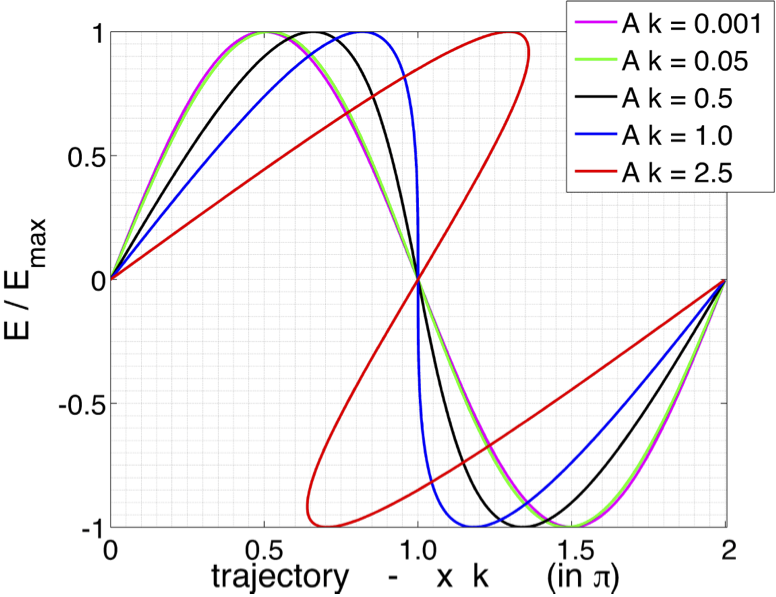
\includegraphics[scale=1]{SahaiThesisPlot.png}
\caption{Plot corresponding to Dawson's derivation of the wave-breaking field [ref. Sahai].}
\label{DawsonCriterionPlot}
\end{figure}
\end{itemize}
\noindent \textbf{Week 3}\\
Meeting Guoxing:
\begin{itemize}
\item We will change $\sigma_{x,y}$, in simulation from $\sigma_{x,y}=0.3 \mu m ~\to~5-10 \mu m$ because the $0.3\mu m$ EuPRAXIA beam parameter gives to high beam density $n_b$, which means that we can't have $n_b\sim n_p$ because the plasma density would have to be too high. We should aim for $n_p\sim 10^{17}-10^{18}\sim n_b$ (standard L/PWFA) parameters. 
EuPRAXIA wants $\sigma_{x,y}$ small because small bunches gives more coherent radiation in undulators. One could expand the beam by letting it propagate freely (expand due to space charge) a distance before reaching the beam dump. 
\item $\text{Run simulations with uniform plasma density for }\left\{\begin{aligned}
&n_p\sim 0.1 n_b \quad &&\text{Non-linear}\\
&n_p\sim  n_b\quad &&\text{Quasi-linear}\\
&n_p\sim 10 n_b\quad &&\text{Linear}
\end{aligned}\right.$ \\
\item Use $\Delta E/E=0.01$ and bunch charge $30~$pC ($5~$fs).\\
\item Estimate necessary simulation propagation length by saturation length using wave-breaking electric field gradient 
$$L_{\text{sat}}\approx \frac{T_0}{eE_{wb}}=\frac{T_0}{e}\frac{e}{m_e c\omega_p}=\frac{T_0}{m_e c}\sqrt{\frac{m_e e\epsilon_0}{e^2n_b}} $$ 
\item Project outline:
\begin{itemize}
\item Uniform plasma with varying $n_b\sim n_p$
\item Vary plasma density profile
\item Test laser to dump head of beam
\item Run simulations for real FlashForward parameters and not the idealized EuPRAXIA parameters.
\end{itemize}
\item  100pC $$n_b=\frac{N_p}{(2\pi)^{3/2} \sigma_y^2\sigma_x}=\frac{6.25\times 10^{8}}{(2\pi)^{3/2} (5\times 10^{-6})^3}\approx 3.2\times 10^{23}~ \text{m}^{-3} $$
$$\Rightarrow ~~eE_{\text{wb}}=\left\{\begin{aligned}
&17 ~\text{GeV/m }&& n_p=0.1 n_b \\
&54 ~\text{GeV/m} && n_p=n_b\\
&172 ~\text{GeV/m} &&n_p=10 n_b
\end{aligned}\right.\quad\Rightarrow ~~L_{sat}(1 ~\text{GeV})=\left\{\begin{aligned}
&5.8 ~\text{cm}&& n_p=0.1 n_b \\
&1.9 ~\text{cm} && n_p=n_b\\
&0.6 ~\text{cm} &&n_p=10 n_b
\end{aligned}\right.$$
$$1 ~\text{GeV beam} ~~\Rightarrow ~~ L_{sat}\sim 2 ~\text{cm}=2*10^4 \mu \text{m} $$
\item  30pC $$n_b=\frac{N_p}{(2\pi)^{3/2} \sigma_y^2\sigma_x}=\frac{1.87\times 10^{8}}{(2\pi)^{3/2} (5\times 10^{-6})^3}\approx 9.5\times 10^{22}~ \text{m}^{-3} $$
$$\Rightarrow ~~eE_{\text{wb}}=\left\{\begin{aligned}
&9.4 ~\text{GeV/m }&& n_p=0.1 n_b \\
&30 ~\text{GeV/m} && n_p=n_b\\
&94 ~\text{GeV/m} &&n_p=10 n_b
\end{aligned}\right.\quad\Rightarrow ~~L_{sat}(1 ~\text{GeV})=\left\{\begin{aligned}
&10.7 ~\text{cm}&& n_p=0.1 n_b \\
&3.4 ~\text{cm} && n_p=n_b\\
&1.1 ~\text{cm} &&n_p=10 n_b
\end{aligned}\right.$$
$$1 ~\text{GeV beam} ~~\Rightarrow ~~ L_{sat}\sim 3.4 ~\text{cm}=3.4*10^4 \mu \text{m} $$


\end{itemize}

\begin{itemize}
\item[\textcolor{MancPurple}{\textbullet}] The HPC application was approved for me and we installed EPOCH on the CSF cluster. The newer version of EPOCH could not be installed so we used an older version (epoch-4.8.3) which compiled without any issues. 
\item[\textcolor{MancPurple}{\textbullet}] I set up trial simulations for the alternative EuPRAXIA beam parameters that we wish to simulate, specifically using $\sigma_{x,y}=5 \mu m$ and $Q=30, 100$ pc. The previous Mphys students ran the 100 pc beam at very narrow energy spread $< 1\%$ and original 0.3 $\mu m$ beam width, we want to see the effect of the wider beam. These were run at the lowest acceptable resolution:
\item[\textcolor{MancPurple}{\textbullet}] I queued simulations on the cluster for the 30 pc beam, this time using the higher resolution suggested by Yangme:
\end{itemize}

\begin{equation}
\omega_p=\sqrt{\frac{4\pi e^2n_0}{me}}
\end{equation}
\subsection*{Density perturbations}
Continuity equation
\begin{equation}
\frac{\partial n}{\partial t}=-\mathbf{\nabla}\cdot (n\vec{v})
\end{equation}
where $n$ is the plasma density and $\vec{v}$ the plasma fluid velocity. Charge conservation.\\
Lorentz force law:
\begin{equation}
m_e\frac{\partial n\vec{v}}{\partial t}=en\left(\vec{E}+\frac{\vec{v}\times \vec{B}}{c}\right)
\end{equation}
Treating the plasma response to a particle beam perturbatively we have $n(r,z,t)=n_0+n_1(r,z,t)$ where $n_0$ is the ion density and $n_1$ the plasma perturbation. We let $\vec{v}, \vec{E}, \vec{B}$ be perturbative responses to the beam. From continuity equation we have
\begin{equation}
\frac{\partial n_0}{\partial t}+\frac{\partial n_1}{\partial t}=-\mathbf{\nabla}\cdot (n_0\vec{v})-\mathbf{\nabla}\cdot (n_1\vec{v}) \quad \Rightarrow \quad \frac{\partial n_1}{\partial t}\approx -n_0\mathbf{\nabla}(\vec{v})
\end{equation}
From the Lorentz force law have
\begin{equation}
m_en_0\frac{\partial (1+n_1/n_0)\vec{v}}{\partial t}\approx en_0(1+n_1/n_0)\vec{E} \quad \Rightarrow \quad  m_e\frac{\partial \vec{v}}{\partial t}\approx e\vec{E}
\end{equation}
which, using Gauss's law, gives
\begin{equation}
\frac{\partial (\mathbf{\nabla}\cdot\vec{v})}{\partial t}\approx \frac{e}{m_e}\mathbf{\nabla}\cdot\vec{E}= \frac{e^2}{m_e}4\pi (n_1+n_b)
\end{equation}
where $n_1+n_b$ is the free charge. Hence
\begin{equation}
\frac{\partial^2 n_1}{\partial t^2}= -n_0\frac{\partial (\mathbf{\nabla}\cdot\vec{v})}{\partial t}=-\frac{ 4\pi n_0e^2}{m_e} (n_1+n_b) 
\end{equation}
which gives
\begin{equation}
\frac{\partial^2 n_1}{\partial t^2}+\omega_p^2n_1=-\omega_p^2n_b
\end{equation}
where the $\omega_p=(4\pi e^2n_0/m_e)^{1/2}$ is the plasma frequency. We can rewrite this expression in the reference frame of the beam.\\
Perturbation due to beam $n\left(r,\xi \right)\to n\left(r,\xi \right)+n_1\left(r,\xi \right)$, use Maxwell's equations and continuity equation.
\begin{equation}
-\frac{1}{k_p^2}\left(\frac{\partial^2 }{\partial \xi^2}+k_p^2\right)n_1\left(r,\xi \right)=n_b\left(r,\xi \right) ~,~~n_1\left(r,\xi<0 \right)=0
\end{equation}
\begin{equation}
\mathcal{L}_{\xi}n_1\left(r,\xi \right)=n_b\left(r,\xi \right) \quad \Rightarrow \quad \mathcal{L}_{\xi}G\left(\xi,\xi'\right)=\delta\left(\xi-\xi'\right)
\end{equation}
\textcolor{red}{where the Green's function obeys the same b.c as the density perturbation, i.e it is continuous across the boundary with a discontinuous derivative across the boundary}
Integrate across discontinuity at $\xi=0$
\begin{equation}
\lim_{\epsilon\to 0}\int_{\xi'-\epsilon}^{\xi'+\epsilon} \mathcal{L}_{\xi}G\left(\xi,\xi'\right)\mathrm{d}\xi=\lim_{\epsilon\to 0}\int_{\xi'-\epsilon}^{\xi'+\epsilon}\delta\left(\xi\right)\mathrm{d}\xi=1 \quad \Rightarrow \quad \lim_{\epsilon\to 0}\left[-\frac{1}{k_p^2}\frac{\partial G}{\partial \xi}\right]^{\xi'+\epsilon}_{\xi'-\epsilon}=1
\end{equation}
Without loss of generality we may set the arrival of the beam to be at $t=0$, such that $\xi'=0$.
\begin{equation}
G\left(\xi,\xi'\right)=-k_p\sin\left(k_p\xi \right)\Theta\left(\xi \right) \quad \Rightarrow \quad n_1\left(r,\xi \right)=\int_{-\infty}^{\infty}G\left(\xi,\xi'\right)n_b\left(r,\xi' \right) \mathrm{d}\xi'
\end{equation}

\begin{equation}
\nabla^2\vec{E}-\frac{1}{c^2}\frac{\partial^2 \vec{E}}{\partial t^2}=\frac{4\pi}{c^2}\frac{\partial \vec{J}}{\partial t}+4\pi\boldsymbol{\nabla}\rho~,
\end{equation}
\begin{equation}
\frac{\partial \vec{J}_p}{\partial t}=\frac{e^2 n}{m_e}\vec{E}~.
\end{equation}
\begin{equation}
\left(\nabla^2-\frac{1}{c^2}\frac{\partial^2}{\partial t^2}-k_p^2\right)E_z=\frac{4\pi}{c}\frac{\partial \rho_b}{\partial t}+4\pi\frac{\partial}{\partial z}\left(\rho_b+\rho_p\right)~,
\end{equation}
where $k_p=\omega_p/c$ is the plasma wave number. To solve this we assume that $E_z$ is radially symmetric and write the Laplace operator in cylindrical polar coordinates, $\nabla^2=\nabla^2_{\perp}+\partial^2_z$, where the transverse component
\begin{equation}
\nabla_{\perp}^2=\frac{1}{r}\frac{\partial }{\partial r}r\frac{\partial }{\partial r} +\frac{1}{r^2}\frac{\partial^2 }{\partial \phi^2} ~.
\end{equation}
Furthermore, the derivation is simplified by working in Fourier transform space, where
\begin{equation}
E_z(\xi)=\frac{1}{2\pi}\int_ {-\infty}^{\infty}\wtilde{E}_z(k)e^{ik\xi}\mathrm{d}k~,
\end{equation}
\begin{equation}
 \left(\frac{\partial^2 }{\partial r^2}+\frac{1}{r}\frac{\partial }{\partial r} -k^2_p\right)\wtilde{E}_z
=4\pi ik_p^2 \frac{k}{k^2-k_p^2}\wtilde{\rho}_b~,
\end{equation}
. This is the Fourier transformed version of equation (\ref{Ez_wave_equation}), Hence by solving this this PDE we can find $E_z$ through an inverse Fourier transform. DDone by finding its Green's function, $G(\vec{r},\vec{r}')$, which in cylindrical coordinate satisfies
\begin{equation}
LG(\vec{r},\vec{r}')=\frac{1}{r}\delta(r-r')\delta(\phi-\phi')\delta(z-z')~,
\end{equation}
where the delta function has been written in cylindrical polar coordinates. Since the PDE is radial we can write the Green's function as
\begin{equation}
G(\vec{r},\vec{r}')=G_r(r,r')\delta(\phi-\phi')\delta(z-z')~,
\end{equation}
which leads to 
\begin{equation}
LG_r(r,r')=\frac{1}{r}\delta(r-r')~,
\end{equation}
where left-hand side is the modified Bessel function of order zero \cite{Jackson1962}. Consequently, the Green's function is formed by linear combinations of the modified Bessel functions of order zero, denoted by $K_0$ and $I_0$: %\todo{Standard Bessel function with complex arguments} the linearly independent, 

which implies that $A_0=-1$ and that
\begin{equation}
G\left(r,r'\right)=- I_0(k_pr)K_0(k_pr')\Theta(r'-r)-I_0(k_pr')K_0(k_pr)\Theta(r-r')~.
\end{equation}
We can thus find $\wtilde{E}_z$ from 
\begin{equation}
\wtilde{E}_z(r,k)=\int_{0}^{\infty}G\left(r,r'\right)f(r',k)r'\mathrm{d}r'~,
\end{equation}
and then perform an inverse Fourier transform to find the co-moving longitudinal wakefield:
%\begin{equation}
%E_z(r,\xi)=\frac{1}{2\pi}\int_ {-\infty}^{\infty}\wtilde{E}_z\left(r,k\right)e^{ik\xi}\mathrm{d}\xi
%\end{equation}
%Doing this yields 
\begin{align}
E_z(r,\xi)&=-{2ik_p^2}\int_{-\infty}^{\infty}\frac{ke^{ik\xi}}{k^2-k_p^2}\mathrm{d}k\int_0^{\infty}G\left(r,r'\right)\wtilde{\rho}_b(r')r'\mathrm{d}r'~.
\label{e_z}
\end{align}
For a known beam distribution $\rho_b(r,\xi)$ (add $\xi$ in all previous expressions?) this expression can be used to compute the resulting longitudinal electric field. We shall now proceed by calculating this for a bi-Gaussian bunch distribution. To do this, we could compute the electric field from the Green's function directly and then carrying out the inverse Fourier transform, or we could choose to first compute the field due to a point-particle and then convolving it with the bi-Gaussian distribution. 
For a known beam distribution $\rho_b(r,\xi)$ this expression can be used to compute the resulting longitudinal electric field. Of particular interest to us is the field induced by the propagation of an electron bunch that is Gaussian in both the transverse and longitudinal directions, a so-called bi-Gaussian bunch. To compute this we follow an approach by Dawson \cite{Katsouleas1987} and first evaluate the field due to a point-particle and then convolve it with our bi-Gaussian driver. We choose a radially symmetric point-particle distribution ${\rho}_{0}(r,\xi)$ to match our Green's function:
\begin{align}
{\rho}_{0}(r,\xi)=-\frac{e}{2\pi r}\delta(r-r')\delta(\xi)~. %\quad \Rightarrow\quad  \wtilde{\rho}_{b_0}(r,k)=\int_ {-\infty}^{\infty}\rho_b(r,\xi)e^{-ik\xi}\mathrm{d}\xi=\frac{e}{2\pi r}\delta(r-r')
\end{align}
Substituting the Fourier transform of this into equation (\ref{e_z}) and performing a contour integrating in k-space yields 
\begin{equation}
E_z(r,\xi)=2ek_p^2\cos(k_p\xi)G\left(r,r'\right)\Theta(\xi)~,
\label{singe-particle-wake}
\end{equation}
where $\Theta(\xi)$ ensures causality is preserved. This is the so called single-particle wake function \cite{Katsouleas1987}. The longitudinal electric field resulting from an arbitrary radially-symmetric source distribution $n_b(r,\xi)$ is now given by convolving the source by the single-particle wake function:
\begin{align}
E_z(r,\xi)=2ek_p^2\int_0^{2\pi}\mathrm{d}\phi  \int_{-\infty}^{\infty} \cos(k_p(\xi-\xi'))\Theta(\xi-\xi')\mathrm{d}\xi' \int_{0}^{\infty}G\left(r,r'\right) n_b(r',\xi')r'\mathrm{d}r'~.
\end{align}
%\begin{equation}
%\wtilde{E}_z(r,k)=-2eik_p^2\frac{k}{k^2-k_p2}G\left(r,r'\right)
%\end{equation}
which satisfies (\ref{diffeq_in_transformspace}), as can be shown by integrating across the discontinuity and taking the limit to zero, and then gives
\textcolor{red}{But my Green's function has a $A=-1$ as constant and not $A=4\pi$ as Bonatto and Gessner}\\The electric force is thus $F_z(r,\xi)=-eE_z(r,\xi)$. 
To compare with simulations and experiments we now choose to convert from CGS to SI units by having $e^{\text{CGS}}\to e^{SI}/\sqrt{4\pi\epsilon_0}$. The longitudinal wakefield in SI units (J/m) is thus
\begin{equation}
E_z(r,\xi)=\frac{e k_p^2}{\epsilon_0} \int_{-\infty}^{\xi} \cos(k_p(\xi-\xi'))\mathrm{d}\xi' \int_{0}^{\infty}G\left(r,r'\right) n_b(r',\xi')r'\mathrm{d}r'~.
\label{longitudinalforce}
\end{equation}
To test the validity of the linear fluid model as well as highlight some key features of the longitudinal wakefield we will calculate this field numerically for a 1 GeV bi-Gaussian bunch with a density of the form
\begin{equation}
n_b(r,\xi)=\frac{N_b}{(2\pi)^{3/2}\sigma_r^2\sigma_{\xi}}e^{-\xi/(2\sigma_{\xi}^2)-r/(2\sigma_{r}^2)}~,
\label{bigaussian}
\end{equation}
\begin{figure}
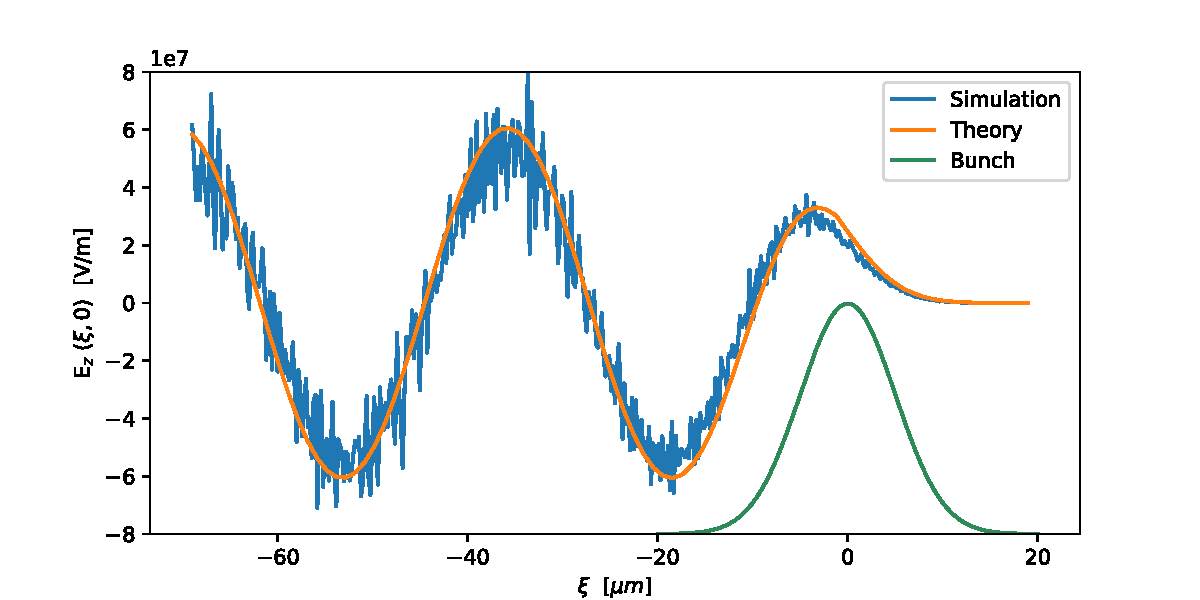
\includegraphics[width=\textwidth]{longitudinal_theory_vs_simulation}
\caption{Mathematica results, integration of longitudinal equation vs simualtion reusults for $n_p=100n_b$, using eupraxia paramaeters. }
\end{figure}
\subsection*{Transverse field}
Panosky-Wenzel theorem:
\begin{equation}
\frac{\partial W_{\perp} }{\partial z}=\frac{\partial W_{\parallel} }{\partial r}~,
\end{equation} 
where, in our case, $W_{\parallel}=E_z$ such that
\begin{equation}
W_{\perp}(r,\xi)=\int \frac{\partial E_z(r,\xi) }{\partial r}\mathrm{d}z~.
\end{equation}
The transverse force on a bi-Gaussian bunch can now by found by applying this expression to the longitudinal single-particle wakefield (\ref{singe-particle-wake}) and then performing the same convolution as above \cite{Katsouleas1987, Mira2017}, which yields 
\begin{figure}
\centering
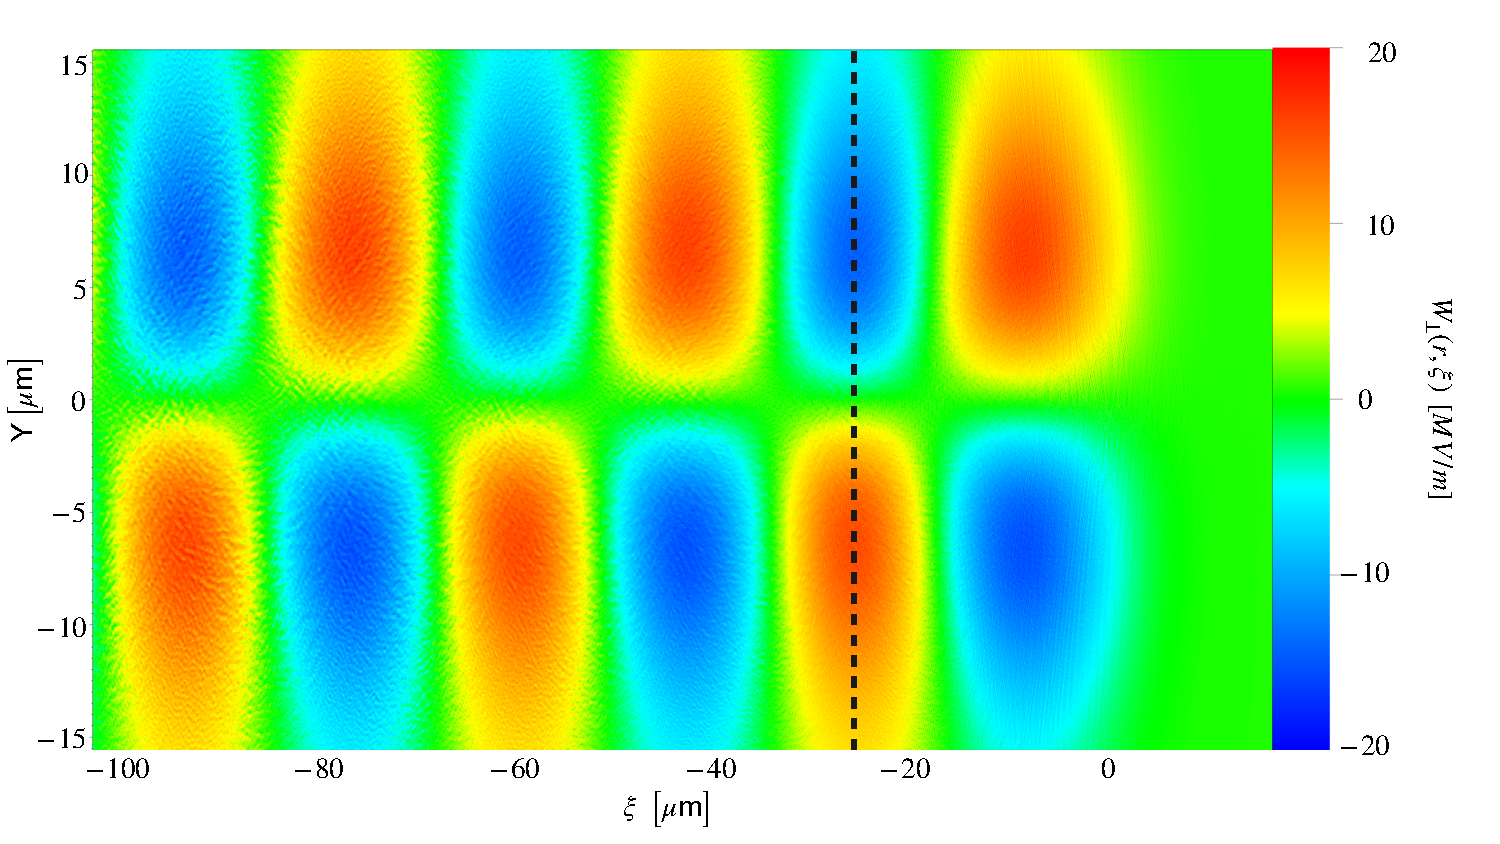
\includegraphics[width=0.8\textwidth]{transverse2d_final}
\caption{\small{Two-dimensional simulation plot of the co-moving transverse wakefield in the linear regime, $n_p=100n_b$, showing successive focusing and defocusing regions. The electron bunch (not shown) is centred on $\xi=0$ and moves to the right.}}
\label{transverse_plot}
\end{figure}
\begin{equation}
W_{\perp}(r,\xi)=\frac{e k_p}{\epsilon_0} \int_{-\infty}^{\xi} \sin(k_p(\xi-\xi'))\mathrm{d}\xi' \int_{0}^{\infty}\frac{\partial G\left(r,r'\right)}{\partial r} \frac{n_b(r',\xi')}{\partial r'}~.
r'\mathrm{d}r'
\label{transverse_wakefield}
\end{equation}
\begin{figure}
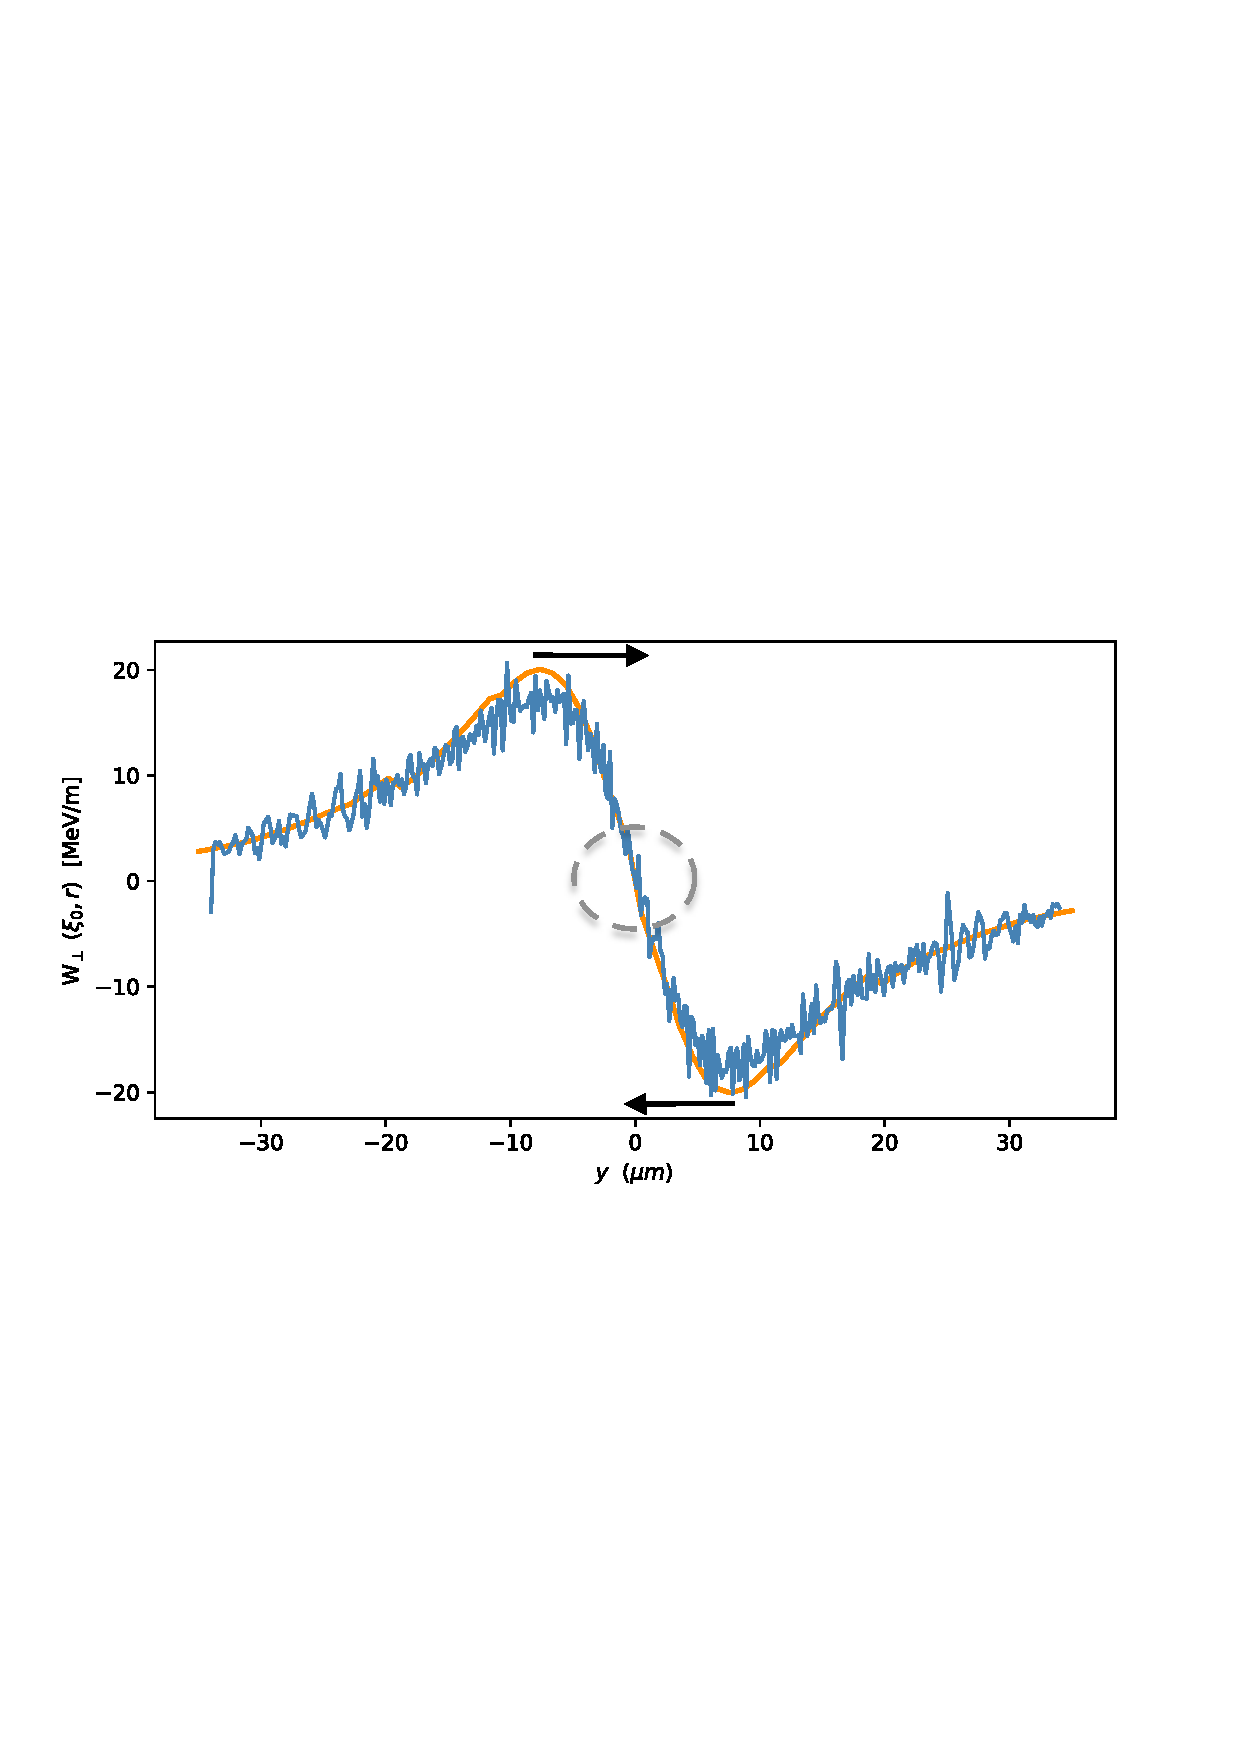
\includegraphics[width=\textwidth]{transverse_theory_vs_sim4}
\caption{Mathematica results, integration of transverse equation vs simualtion reusults for $n_p=100n_b$, using eupraxia paramaeters. }
\end{figure}
\clearpage
\section*{Non-linear Regime} 
\subsection*{Wave-breaking field}
\underline{Dawson's derivation} [Note: The wave-breaking field does not represent the onset of the non-linear regime but the highest achievable field in the non-linear regime.]
We consider a simple 1D linear non-relativistic electron sheet model first used by Dawson \citep{Dawson1959} to show the breakdown of the linear model (\textcolor{red}{correct?}). Consider the plasma being made up of thin sheets of ions and electrons. A sheet at equilibrium position $z=z_0$ is then displaced by $\eta_0(z_0)$, where the displacement is set as function of the equilibrium position for full generality, to a new position $z=z_0+\eta_0$. The displaced sheet reveals a positive surface charge density $\sigma=en_0\eta_0$, where $n_0$ is the electron charge density in the plasma. This sets up a restoring electric field which we find using Gauss's law to be $E_{\text{res}}=4\pi n_0e\eta_0$ which yields a restoring force
\begin{equation}
 m_e\frac{\partial^2\eta_0}{\partial t^2}=-eE_{\text{res}}=-4\pi n_0e^2\eta_0=-\omega_p^2\eta_0
 \end{equation} 
 with solutions 
 \begin{equation}
 \eta_0(z_0,t)=A_1(z_0)\cos(\omega_p t)+A_2(z_0)\sin(\omega_p t)
 \end{equation}
The phenomena of wave breaking can be shown by considering another electron sheet at an equilibrium position $z_1=z_0+\Delta z_0$ at a distance $\Delta z_0$ away from the first sheet. This sheet is then displaced by $\eta_1$ to a new position $z^{*}_1=z_0+\Delta z_0+\eta_1$. The linear model is valid provided that there are no electron trajectories intersect one another in the plasma [ \textcolor{red}{is this correct? Why does the model break down?} ]. Hence the model is valid provided that $z^{*}_1-z_0>z-z_0$ which implies that we must have
\begin{equation}
\Delta z_0+\eta_1>\eta_0~,
\label{eta_ineq}
\end{equation}
for all $\Delta z_0\in \mathbb{R}$, to sustain plasma oscillations in the linear model. We now consider  the limit as $\Delta z_0\to 0$ for the expression 
\begin{equation}
\frac{\partial \eta}{\partial x_0}=\lim_{\Delta z_0\to 0}\frac{\Delta \eta}{\Delta z_0}=\lim_{\Delta z_0\to 0}\left(\frac{\eta_1-\eta_0}{\Delta z_0}\right)>\lim_{\Delta z_0\to 0}\left(\frac{\eta_0-\Delta z_0-\eta_0}{\Delta z_0}\right)=-1
\end{equation}
which simplifies to
\begin{equation}
\frac{\partial \eta}{\partial z_0}>-1
\label{no_crossing}
\end{equation}
where the inequality is introduced using Eq. (\ref{eta_ineq}). We now consider the special case where $A_1(z_0)=A\sin(k_pz_0)$ and $A_2(z_0)=0$. This is a valid solution since $\sin(k_pz_0)$ is single-valued for all $k_p,x_0\in\mathbb{R}$. This particular solution is chosen to highlight the breadown of the electric field, and is motivated by ([\textcolor{red}{what?}]) the solution we found for the electric field in section 2. Applying the no-crossing criterion in Eq. \ref{no_crossing} to $\eta=\eta_0(z_0,t)$ yields
\begin{equation}
\frac{\partial \eta_0}{\partial z_0}=Ak_p\cos(k_pz_0)>-1 \quad \Leftrightarrow \quad Ak_p\leq 1
\end{equation}
which gives the maximum amplitude as $A_{max}=1/k_p$. Hence the maximum restoring electric field $E_{max}\equiv E_{\text{wb}}=4\pi n_0/k_p$ is given by
\begin{equation}
E_{\text{wb}}=\frac{m_ev_p\omega_p}{e}
\end{equation}
the so-called \textit{wave-breaking field}. To further show how this breaks the linear model we consider the effect on the electric field up to and past the wave-breaking limit. As above we have, 
\begin{equation}
z=z_0+\eta_0=z_0+A\sin(k_p z_0)
\label{dawson_z}
\end{equation}
and 
\begin{equation}
E=4\pi n_0e A\sin(k_p z_0)
\label{dawson_E(z)}
\end{equation}
from which we want to find the electric field as a function of $z$. We can do this by numerically solving Eq. \ref{dawson_z} for $z_0$ in a range of $z$ values given fixed values of $A$. The gives $z_0=z_0(z,A)$ which can be substituted into Eq. \ref{dawson_E(z)} to give $E=E(z,A)$, the result of which is shown in Fig. \ref{DawsonCriterionPlot}. From this we conclude that the electric field is no longer single-valued for $A>1/k_p$, i.e past the electric field's wave-breaking amplitude, which signifies a breakdown of the linear model.

\clearpage
\section{Particle interactions with matter}
Conventional beam dumps work by stochastic interactions of the beam with the dense medium [hanahoe 6.5]
\subsection{Bohr-Fermi-Bethe-Bloch Theory}
Bethe-Bloch forumla:
\begin{equation}
-\expval{\frac{\mathrm{d}U}{\mathrm{d}s}}_{\text{ion}}=\frac{4\pi e^4n_{e,m}}{m_ec^2\beta^2}\left[\ln\left(\frac{2m_e\gamma^2v^2}{I}\right) -\beta^2\right]
\end{equation}

\subsection{Collective Plasma Deceleration -- Non-Linear regime }

\begin{equation}
-\left(\frac{\mathrm{d}E}{\mathrm{d}z}\right)_{\text{coll-wave-break}}=F_e=eE_{wave-break}=m_e c\omega_{p}\left(\frac{n_b}{n_e}\right)
\end{equation}

What is the wave-breaking electric field?



\subsection{Collective Plasma Deceleration -- Linear regime }
Based on the work of Lu et. al \citep{Lu2006}, wherein it was shown that the predictions from the linear models perform well even in the non-linear regime, it is of interest to compute the energy loss in the linear regime. This follows the analysis by Bonatto et al. \citep{Bonatto2016}.\\
The energy loss of a bunch is due to the work carried out by the longitudinal electric field $E_z$, neglecting effects such as bremsstralung etc. The rate of energy change with propagation distance of a particle at position $(r,\xi)$ in the bunch after travelling is given by the force exerted on the particle by the longitudinal electric field:
\begin{equation}
\frac{\mathrm{d}U_p}{\mathrm{d}s}=-eE_z(r,\xi)
\end{equation}
where we have assumed that there occurs no modulation of the particle bunch as it traverses the plasma, hence the electric field is only a function of the position in the bunch $E_z(r,\xi)$ and not the propagation distance $s$. Integrating over the propagation distance then gives the energy of one particle in the beam at position $(r,\xi)$ after travelling a distance s:
\begin{equation}
U_e(r,\xi,s)=U_e(r,\xi,0)-seE_z(r,\xi)
\end{equation}
from which multiplication by the beam number density $n_b(r,\xi)$ and integration over the volume of the bunch gives the total energy of all particles in the bunch after propagation distance s
\begin{equation}
U(s)=\int  U_e(r,\xi,0)n_b(r,\xi)r\mathrm{d}r\mathrm{d}\xi\mathrm{d}\phi-se\int E_z(r,\xi)n_b(r,\xi)r\mathrm{d}r\mathrm{d}\xi\mathrm{d}\phi
\end{equation}
where $\mathrm{d}V=r\mathrm{d}r\mathrm{d}\xi\mathrm{d}\phi$ [I think].
\subsection{Notes Bonatto}
Rate of change due to the longitudinal electric field acting on an electron beam, i.e position beam in the decelerating region of the wakefield.\\
"the beam only experiences its self-excited wakefield."\\
In the passive beam dump, are we essentially slowing down a "drive bunch" without having a witness bunch behind to get accelerated?\\
It is probaly better to use gamma as in Bonatto's paper, to make it easier to explain total beam energy integral. Basically integrate over all particles.\\
\\
$U=\gamma m_ec^2$
\begin{equation}
-\frac{\mathrm{d}U}{\mathrm{d}s}=(F_e)_z=eE_z
\end{equation}
where $s$ is the distance travelled in the plasma and $U$ is the energy of a particle in the beam at position $\xi$. 
for ultra relativistic beams, $\beta\sim 1$, the longitudinal electric field is a function of the position along the bunch $\xi=z-ct$ and not $z$ explicitly. 
\begin{equation}
U(s,\xi)=U_0-esE_z(\xi)
\end{equation}
The total energy of the beam after travelling a distance $s$ is then found by integrating across all the particles in the beam, which is integrating across $\xi$ since analysis is in 1-D.
\begin{equation}
\mathcal{U}(s)=U_0\int_{-\infty}
\end{equation}

We will proceed by calculating the gamma factor of a given particle in the beam who's energy we wish to compute.
\begin{equation}
\gamma(s,\xi)=\gamma_0-esE_z(\xi)
\end{equation}
\noindent \textbf{Week 4}\\
\begin{itemize}
\item[\textcolor{MancPurple}{\textbullet}] Analysed the simulation data for the low resolution 30 pc beam at 5 $\mu m$ width and RMS length. The beam was propagated for 2 cm, which is the calculated saturation length for the quasilinear simulation. The resulting energy of the beam vs. spatial extent of the beam were generated and compiled into a video using a python script I wrote. The results after 2 cm are shown below:
\begin{figure}[!ht]
\centering
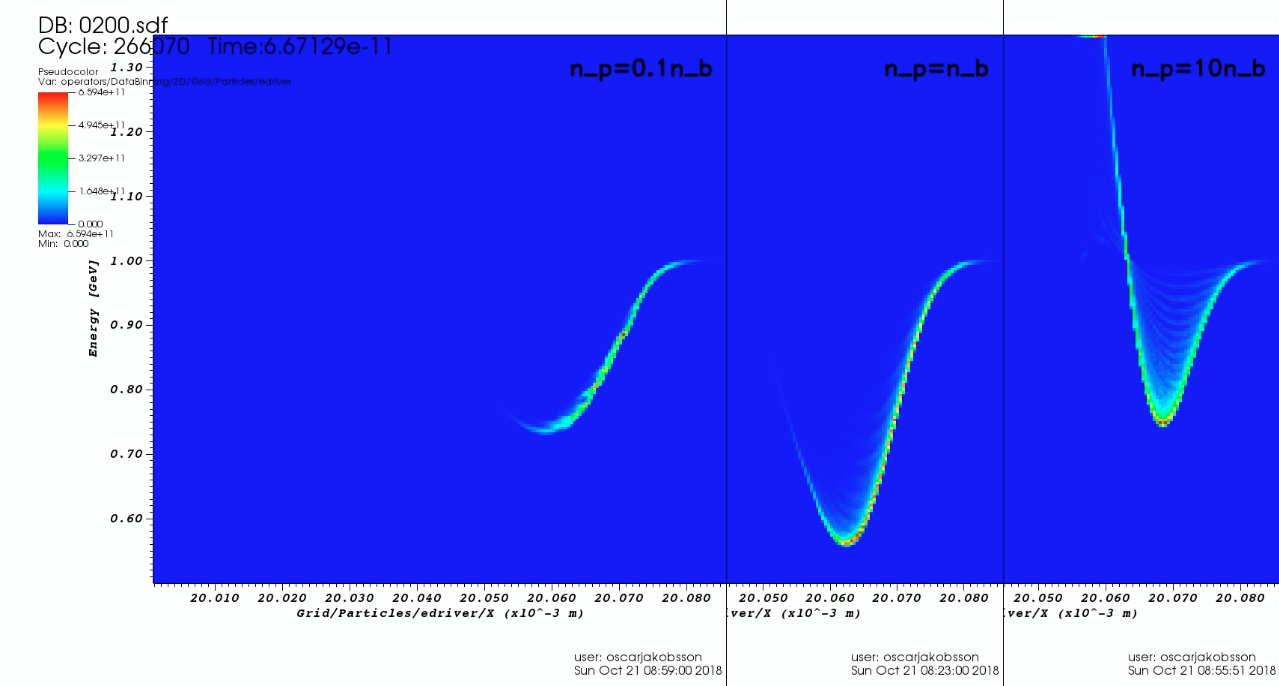
\includegraphics[scale=0.3]{simulation30pc}
\end{figure}
\item[\textcolor{MancPurple}{\textbullet}] By integrating energy histograms using VisIt's query('Integrate') function in a Python script the energy decrease was computed as a function of propagation distance for the 3 cases above:
\begin{figure}[!ht]
\centering
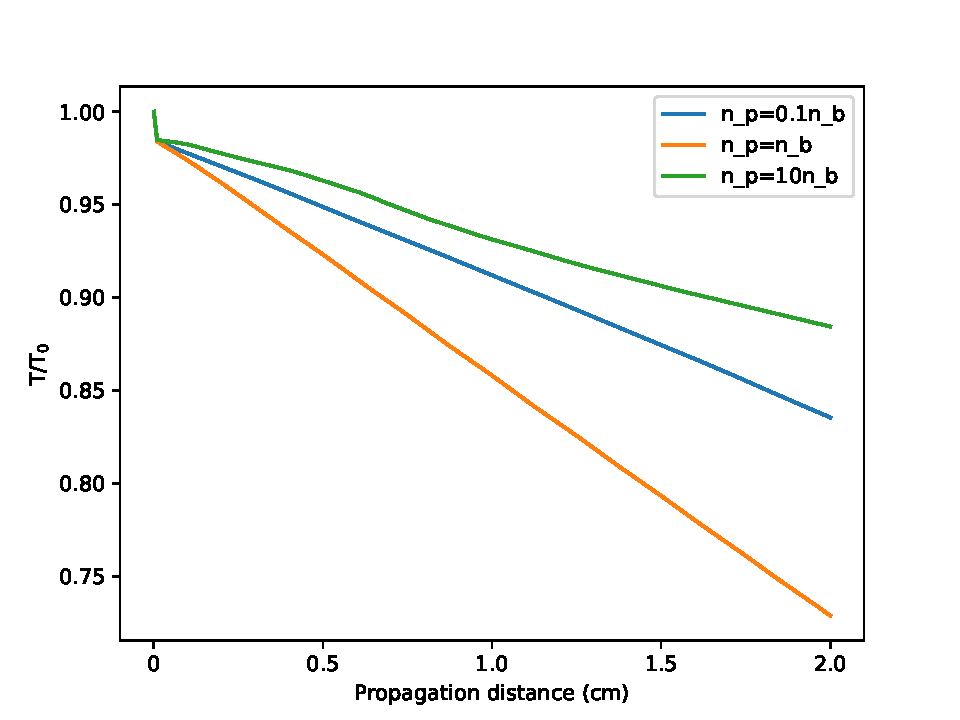
\includegraphics[scale=0.8]{EnergyDecrease30pc.pdf}
\end{figure}
\item[\textcolor{MancPurple}{\textbullet}] The varying plasma density was tried in EPOCH by doing some test simulation. This will be set up and run next week. 
\end{itemize}
\newpage 



\newpage
\section*{Propagation Uniform plasma}
\begin{figure}[!ht]
\centering
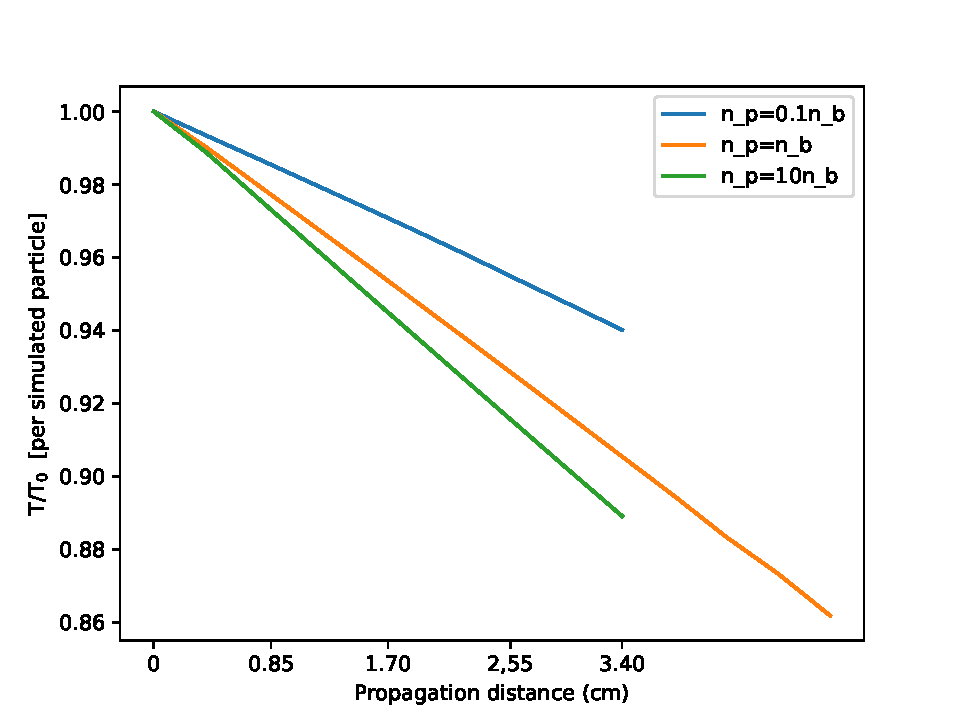
\includegraphics[width=0.75\textwidth]{Energy30pc_per_particle_past_sat_length.pdf}
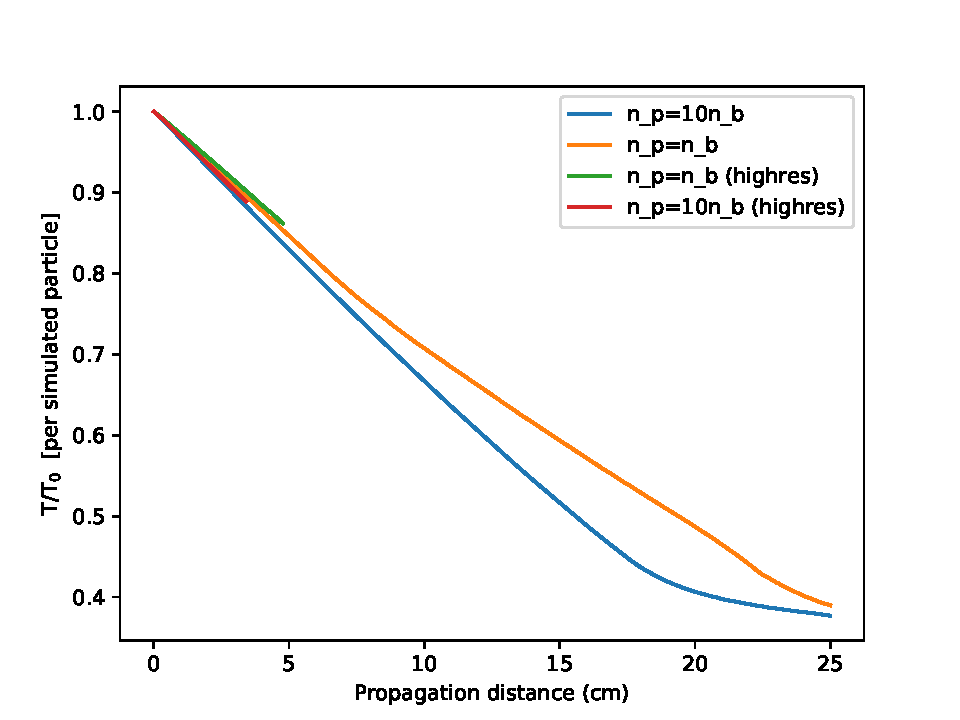
\includegraphics[width=0.75\textwidth]{Energy30pc_per_particle_lowres.pdf}
\end{figure}
\begin{figure}[!ht]
\centering
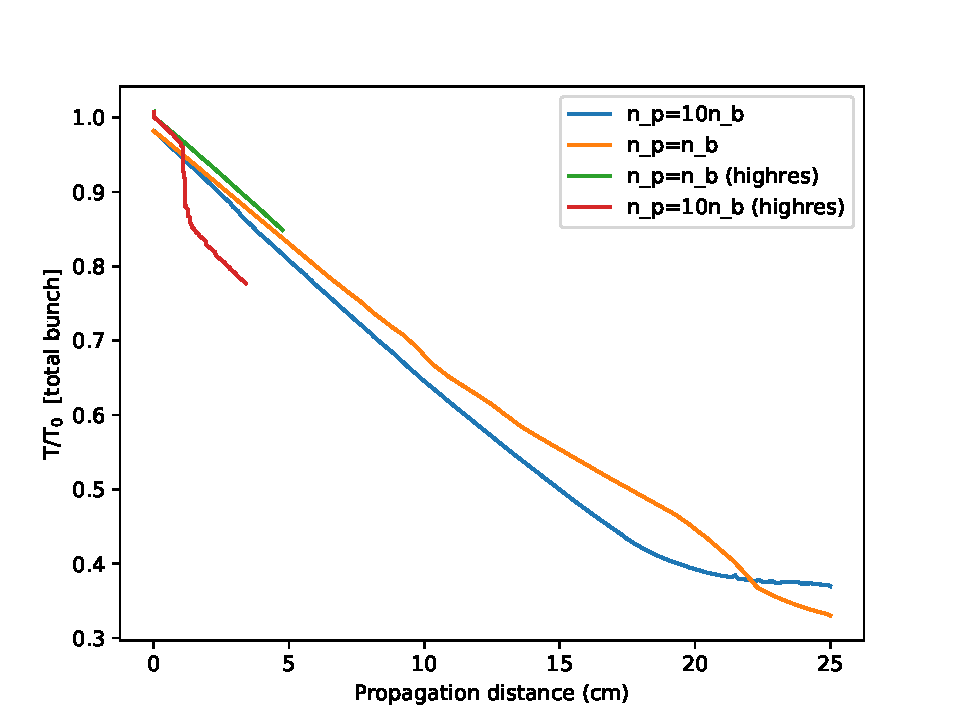
\includegraphics[width=0.78\textwidth]{Energies30pc_lowres.pdf}
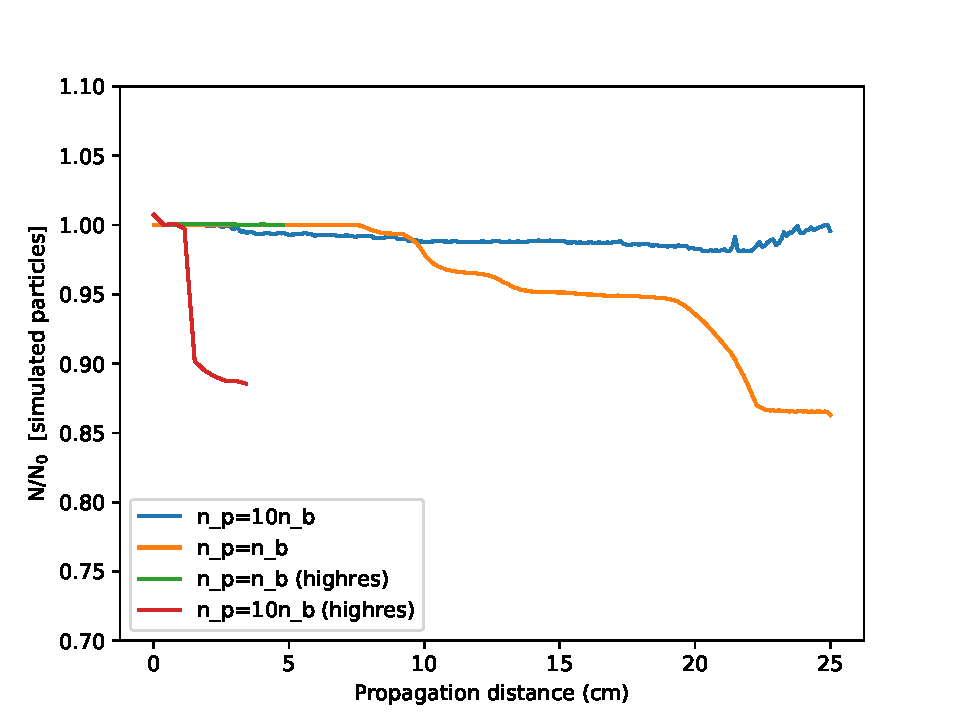
\includegraphics[width=0.78\textwidth]{Particles30pc_lowres.pdf}
\end{figure}


\clearpage
\begin{figure}[!ht]
\centering
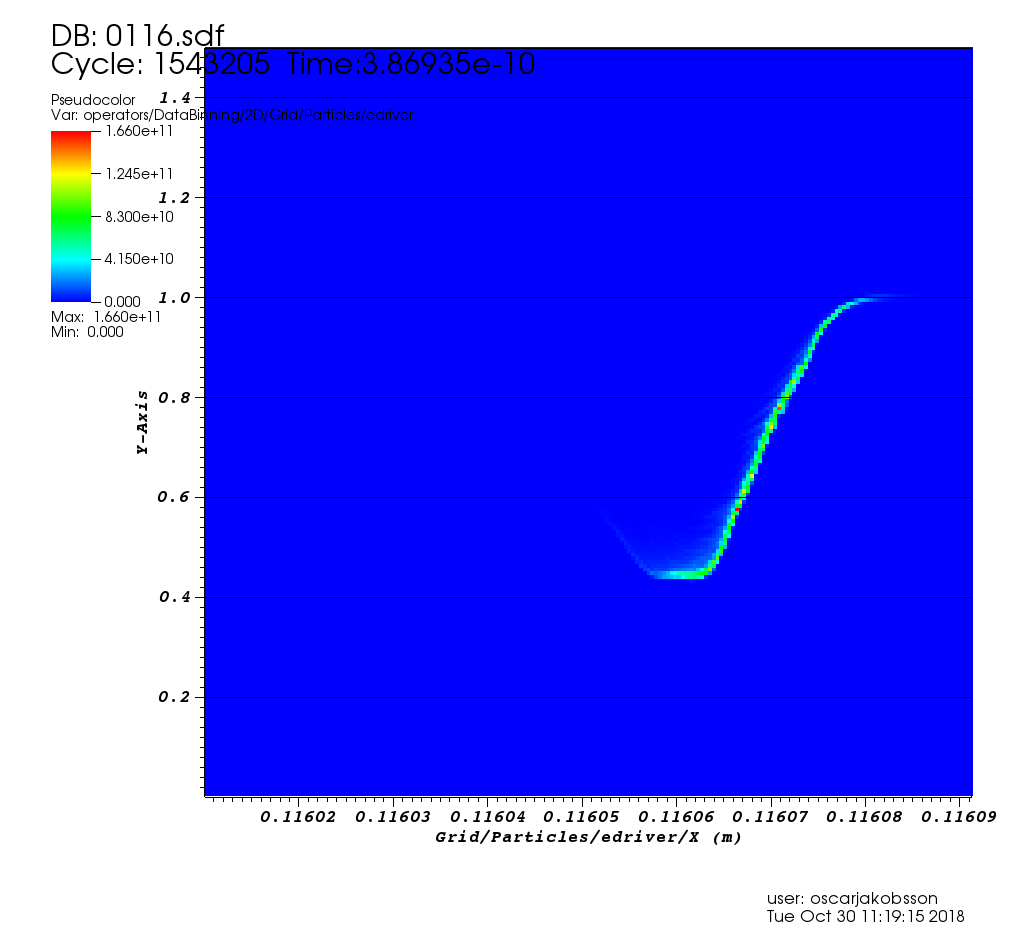
\includegraphics[width=0.49\textwidth]{visit0016.png}
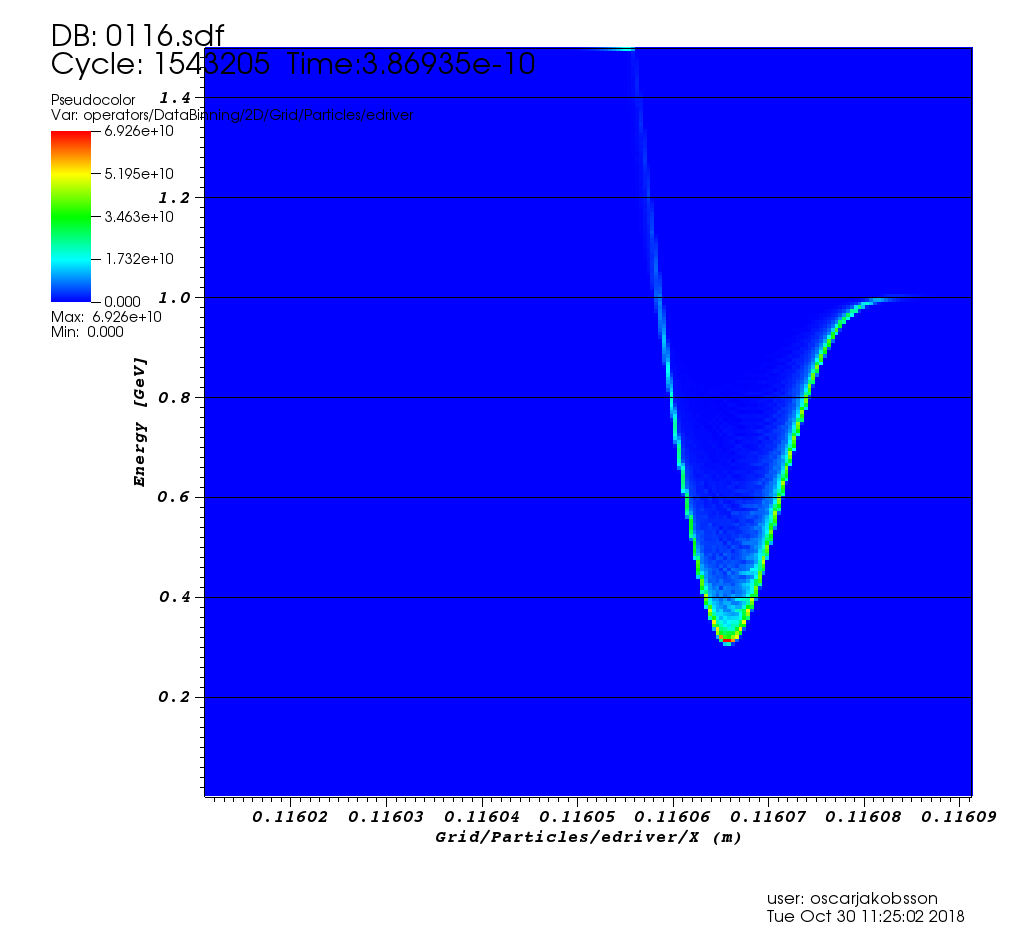
\includegraphics[width=0.49\textwidth]{visit0012.png}
\caption{\textcolor{Orange2}{\textbf{(Left)}}{: Energy distribution for quasilinear case after propagating 11.6 cm} \textcolor{blue}{\textbf{(Right)}}{: Energy distribution for linear case after propagating 11.6 cm.}}
\end{figure}
\begin{figure}[!ht]
\centering
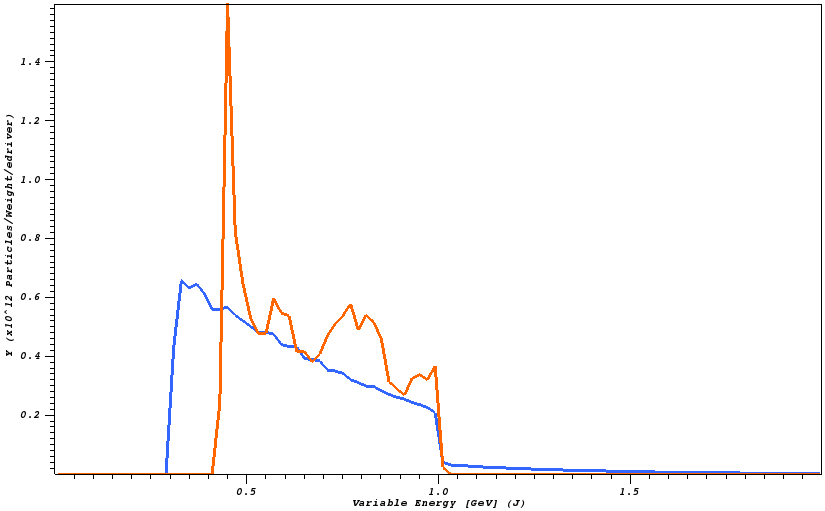
\includegraphics[width=0.9\textwidth]{visit0019.png}
\caption{\textcolor{Orange2}{\textbf{(1)}}{: Quasilinear $n_p=n_b$ after 11.6 cm.} \textcolor{blue}{\textbf{(2)}}{: Linear $n_p=10n_pb$ after 11.6 cm.}}
\end{figure}

\newpage
\begin{figure}[!ht]
\centering
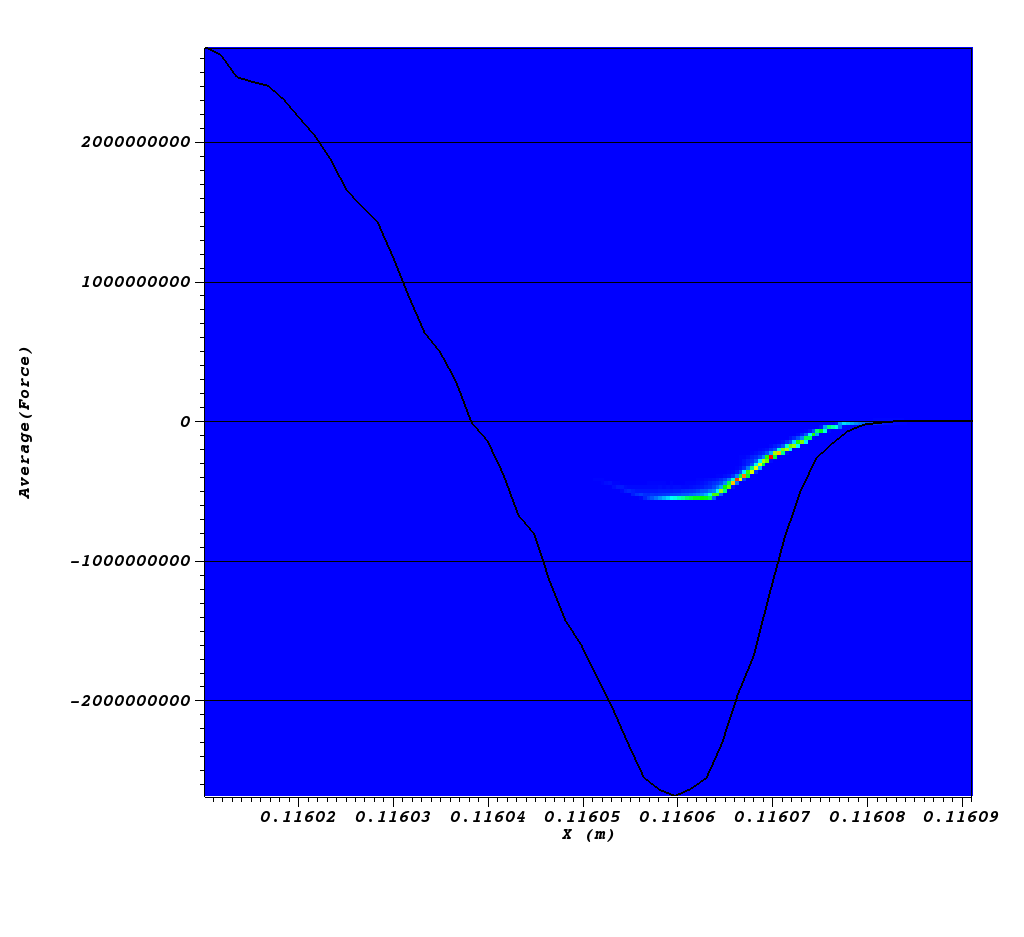
\includegraphics[width=0.6\textwidth]{quasi_energy_force.png}\\
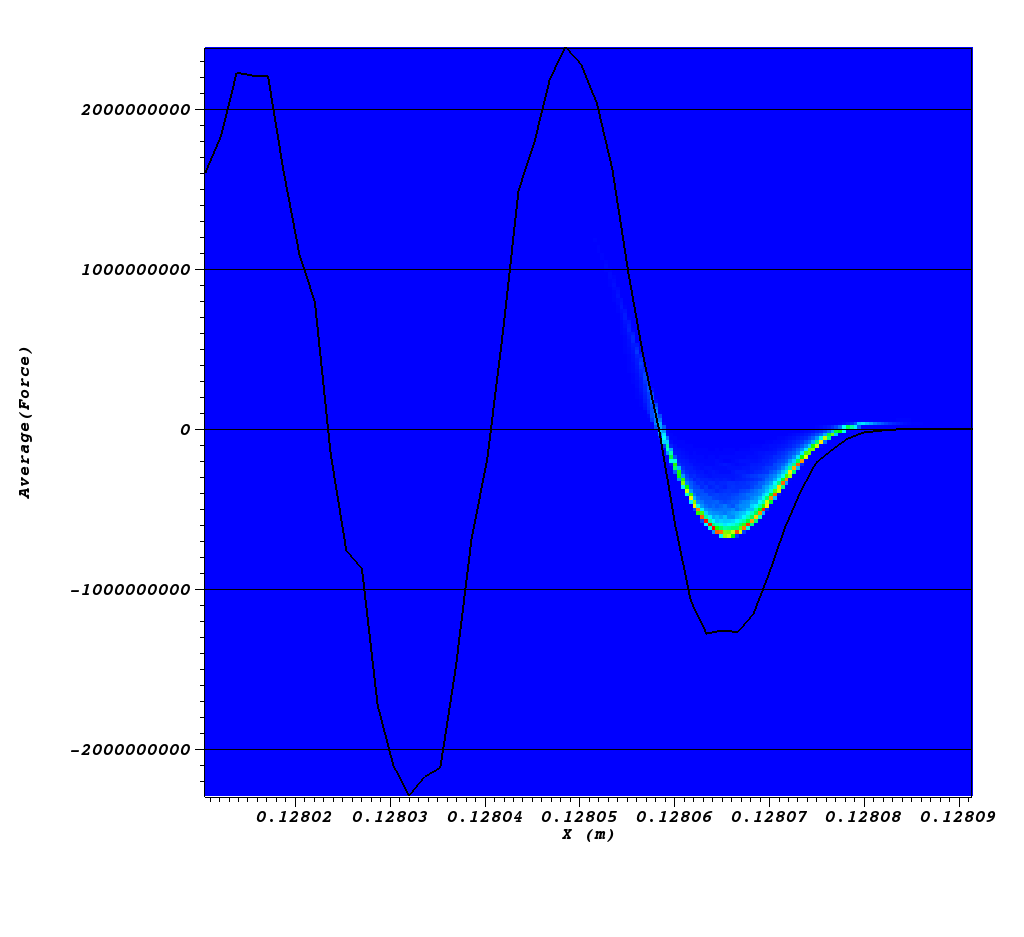
\includegraphics[width=0.6\textwidth]{linear_energy_force.png}
\caption{{\textbf{(Left)}}{: Energy distribution with force for quasilinear case after propagating 11.6 cm} {\textbf{(Right)}}{: Energy distribution with force for linear case after propagating 11.6 cm.}}
\end{figure}

\newpage
\noindent Propagation Uniform plasma.
\begin{figure}[!ht]
\centering
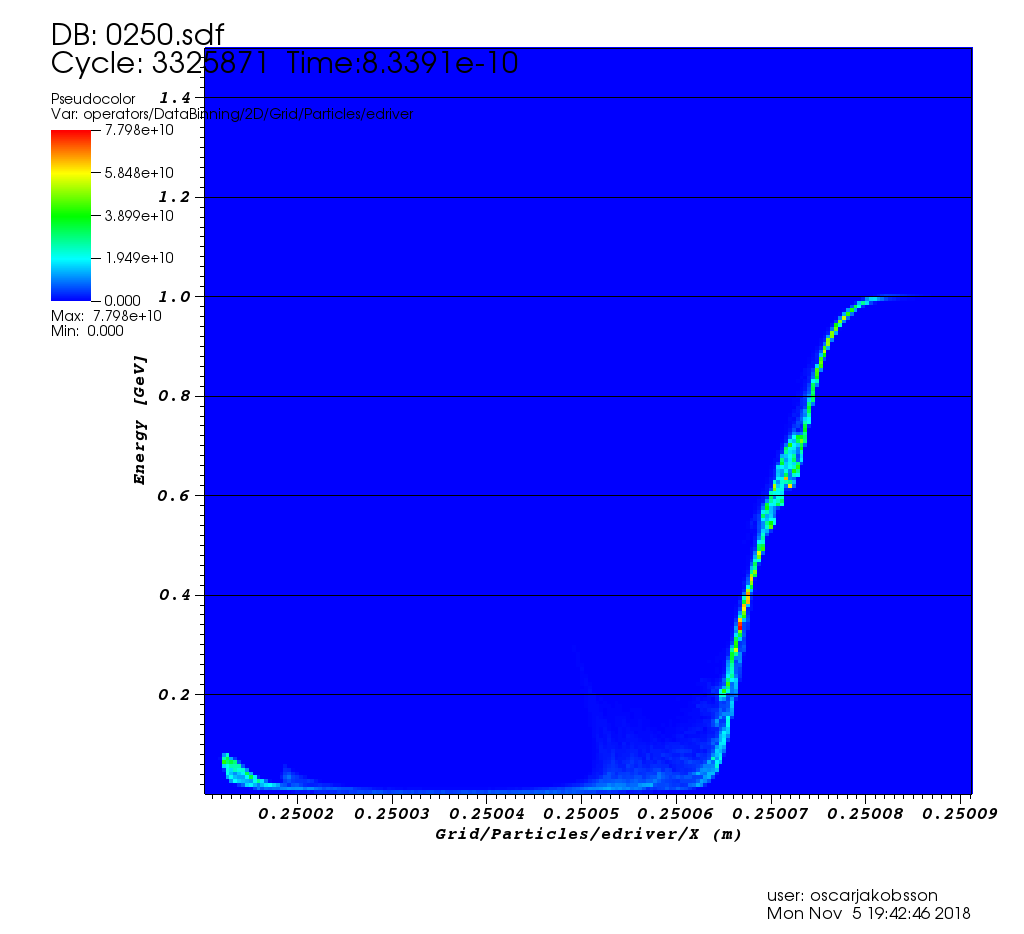
\includegraphics[width=0.49\textwidth]{visit0035.png}
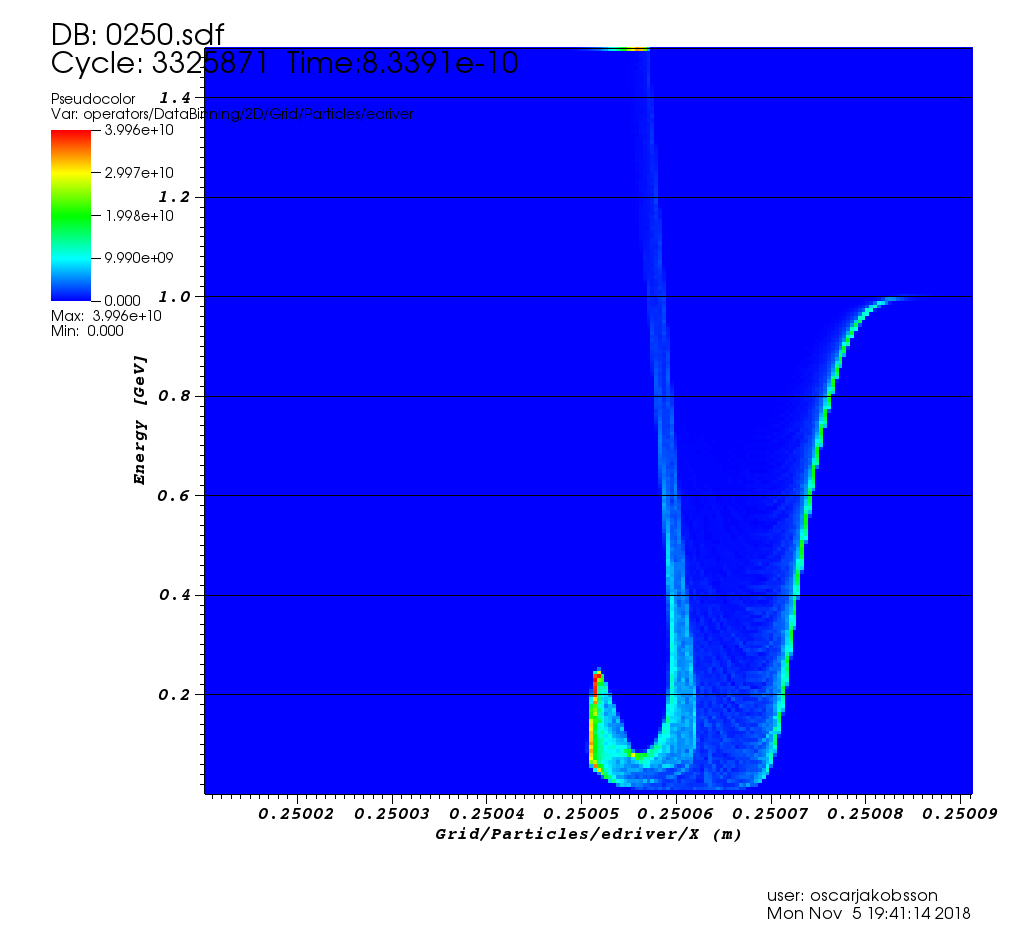
\includegraphics[width=0.49\textwidth]{visit0033.png}
\caption{\textcolor{Orange2}{\textbf{(Left)}}{: Energy distribution for quasilinear case after propagating 25 cm} \textcolor{blue}{\textbf{(Right)}}{: Energy distribution for linear case after propagating 25 cm.}}
\end{figure}
\begin{figure}[!ht]
\centering
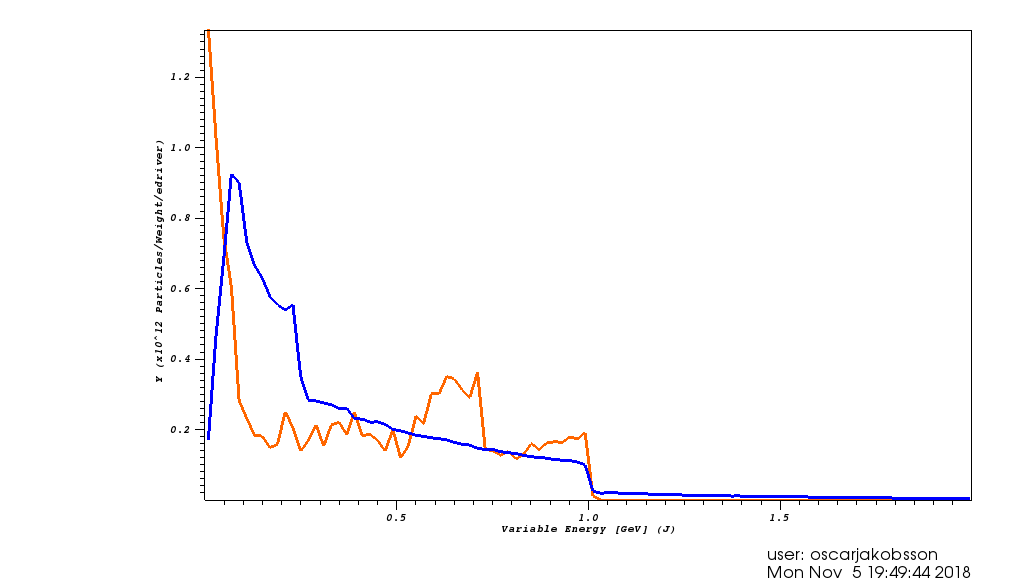
\includegraphics[width=0.9\textwidth]{visit0037.png}
\caption{\textcolor{Orange2}{\textbf{(1)}}{: Quasilinear $n_p=n_b$ after 25 cm.} \textcolor{blue}{\textbf{(2)}}{: Linear $n_p=10n_pb$ after 25 cm.}}
\end{figure}
\begin{figure}[!ht]
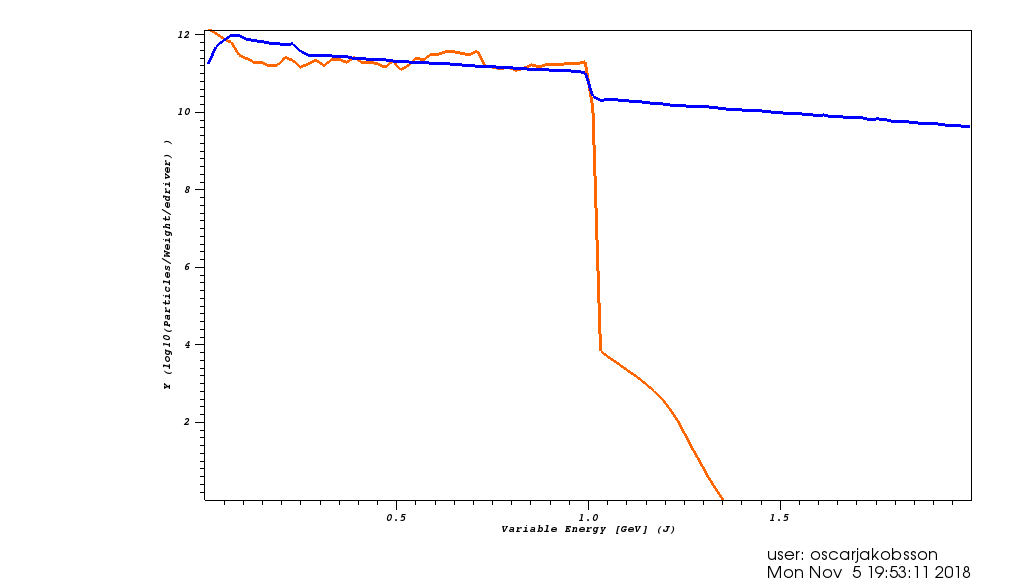
\includegraphics[width=0.9\textwidth]{visit0038.png}
\caption{\textcolor{Orange2}{\textbf{(1)}}{: Quasilinear $n_p=n_b$ after 25 cm.} \textcolor{blue}{\textbf{(2)}}{: Linear $n_p=10n_pb$ after 25 cm.}}
\end{figure}
\begin{figure}[!ht]
\centering
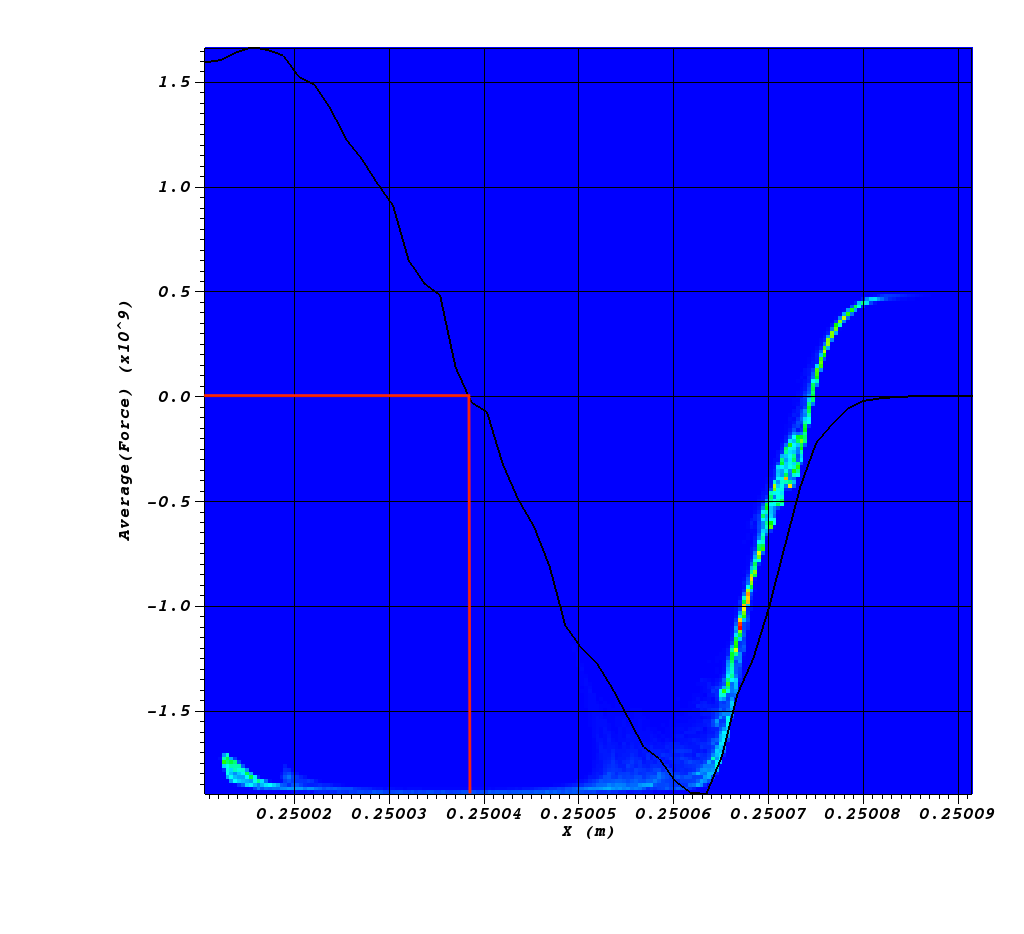
\includegraphics[width=0.49\textwidth]{visit0040.png}
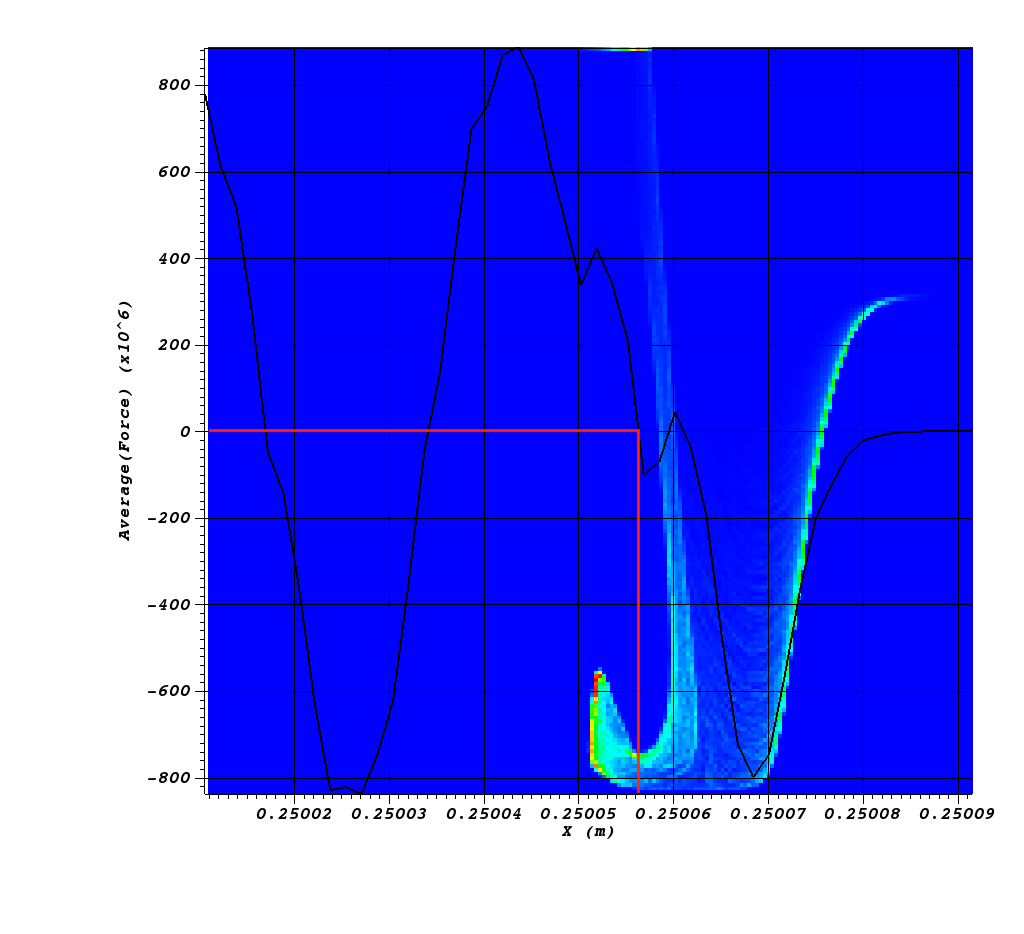
\includegraphics[width=0.49\textwidth]{visit0042.png}
\caption{\textcolor{Orange2}{\textbf{(Left)}}{: Energy distribution with force for quasilinear case after propagating 25 cm} \textcolor{blue}{\textbf{(Right)}}{: Energy distribution with force for linear case after propagating 25 cm}.}
\end{figure}
\clearpage

\begin{figure}[!ht]
\centering
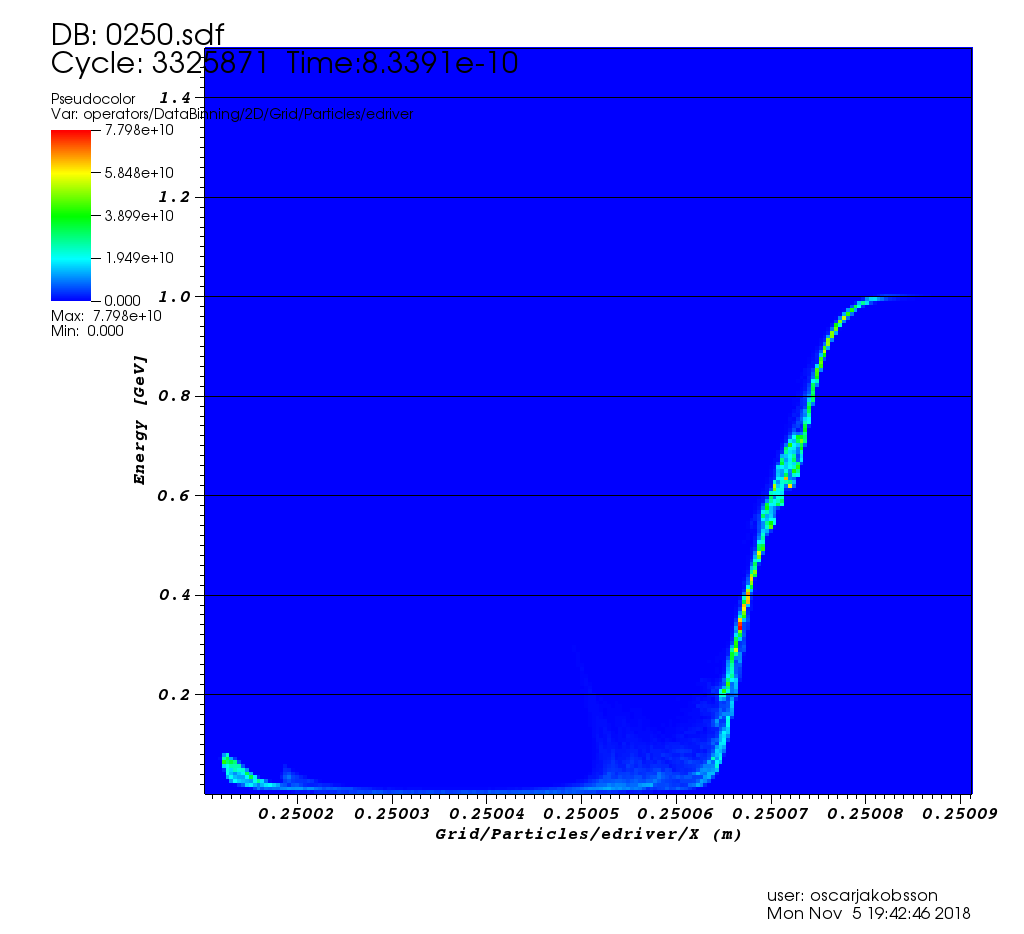
\includegraphics[width=0.49\textwidth]{visit0035.png}
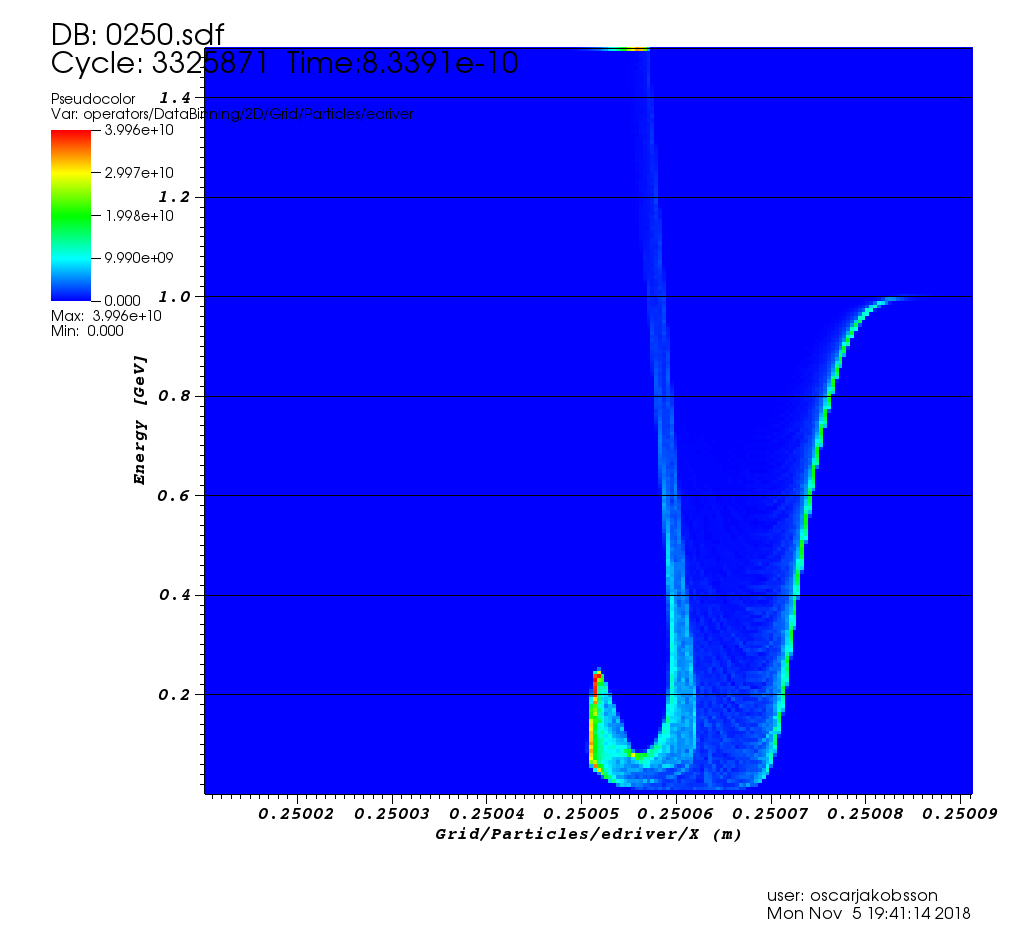
\includegraphics[width=0.49\textwidth]{visit0033.png}
\caption{\textcolor{Orange2}{\textbf{(Left)}}{: Energy distribution for quasilinear case after propagating 25 cm} \textcolor{blue}{\textbf{(Right)}}{: Energy distribution for linear case after propagating 25 cm.}}
\end{figure}
\begin{figure}[!ht]
\centering
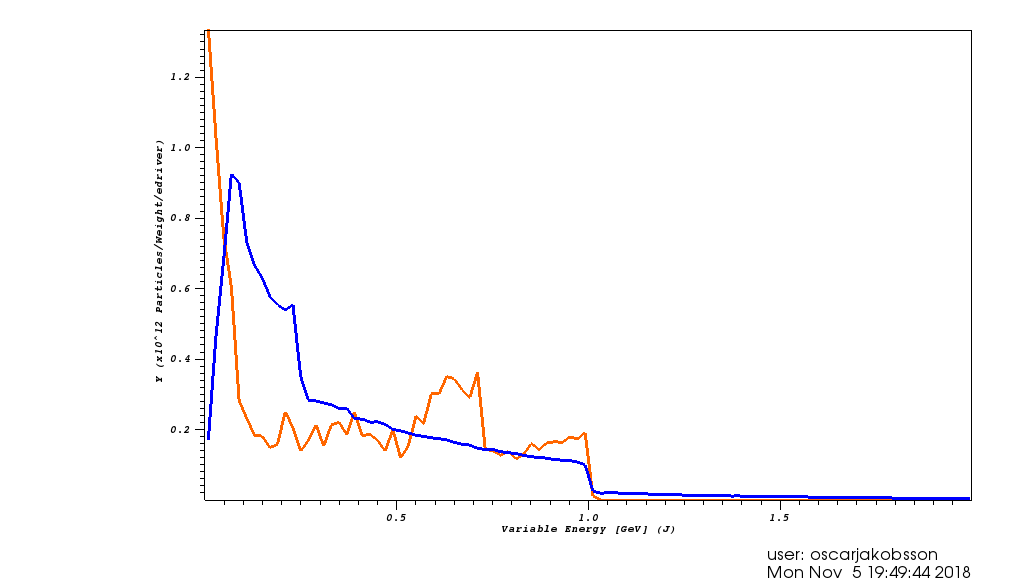
\includegraphics[width=0.9\textwidth]{visit0037.png}
\caption{\textcolor{Orange2}{\textbf{(1)}}{: Histogram energy distribution for quasilinear $n_p=n_b$ after 25 cm.} \textcolor{blue}{\textbf{(2)}}{: Histogram energy distribution for linear $n_p=10n_pb$ after 25 cm.}}
\end{figure}
\clearpage

\begin{figure}[!ht]
\centering
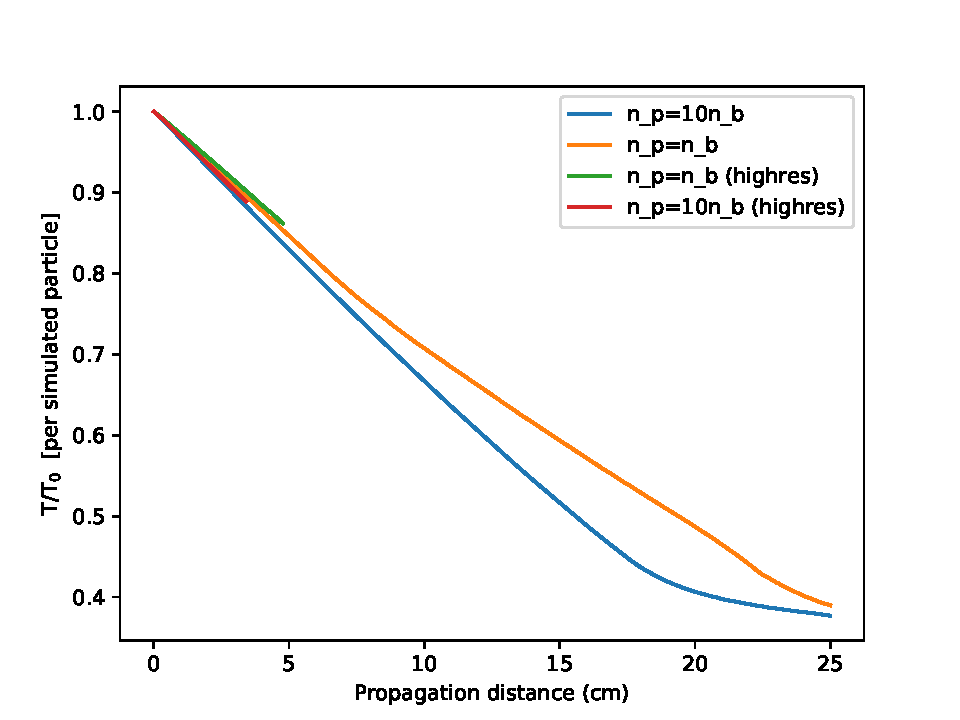
\includegraphics[width=0.75\textwidth]{Energy30pc_per_particle_lowres.pdf}
\end{figure}


\begin{figure}[!ht]
\centering
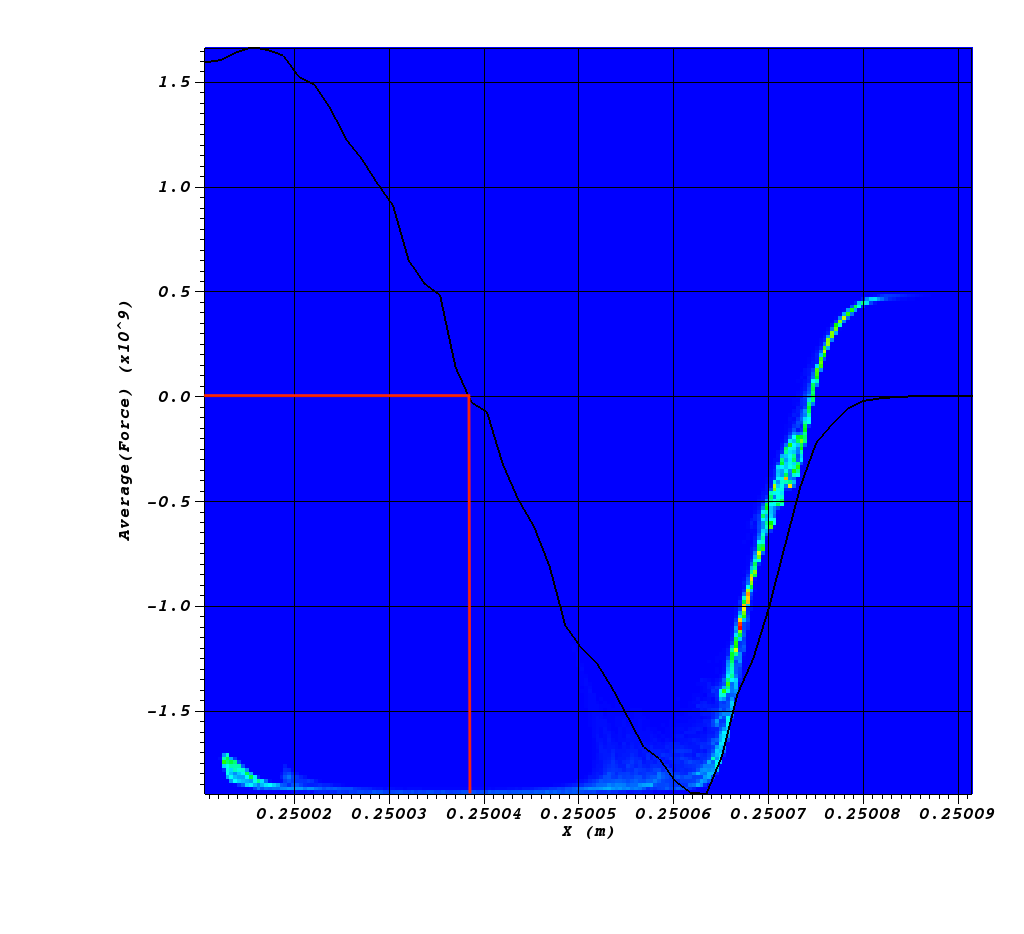
\includegraphics[width=0.49\textwidth]{visit0040.png}
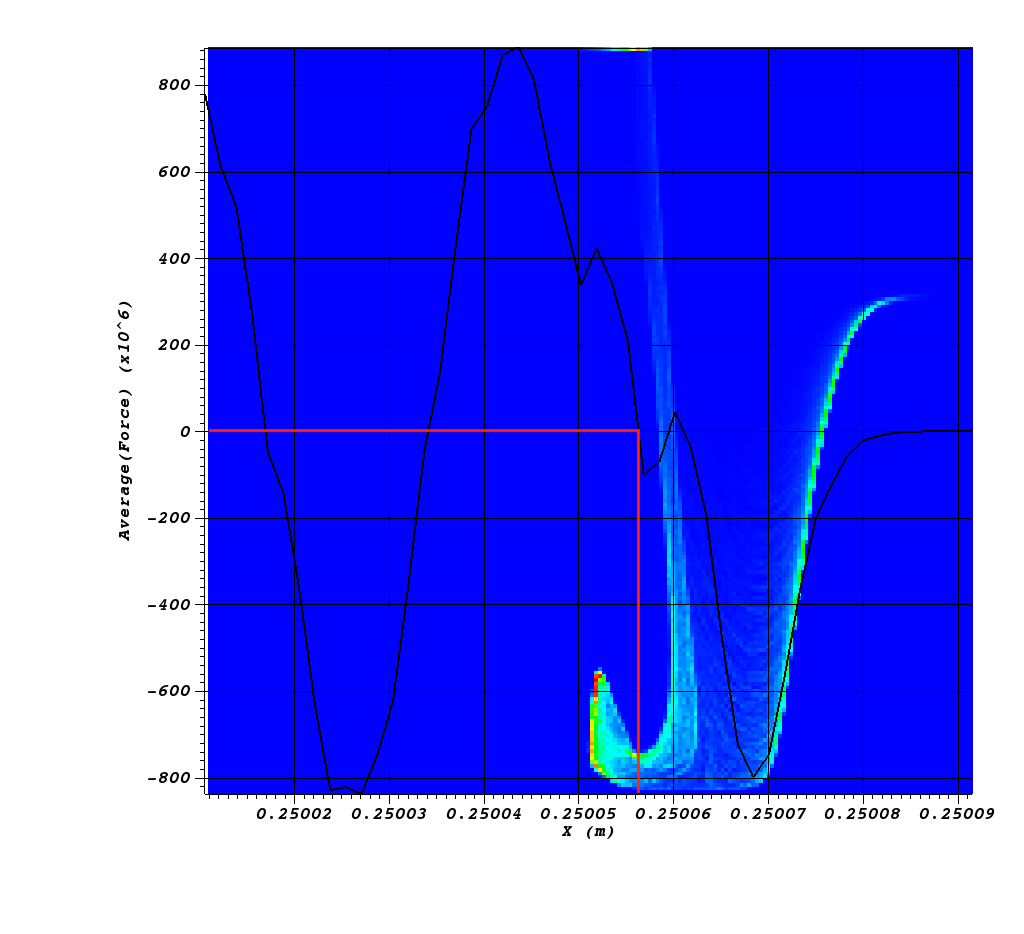
\includegraphics[width=0.49\textwidth]{visit0042.png}
\caption{\textcolor{Orange2}{\textbf{(Left)}}{: Energy distribution with force for quasilinear case after propagating 25 cm} \textcolor{blue}{\textbf{(Right)}}{: Energy distribution with force for linear case after propagating 25 cm}.}
\end{figure}
\clearpage
\begin{figure}[!ht]
\centering
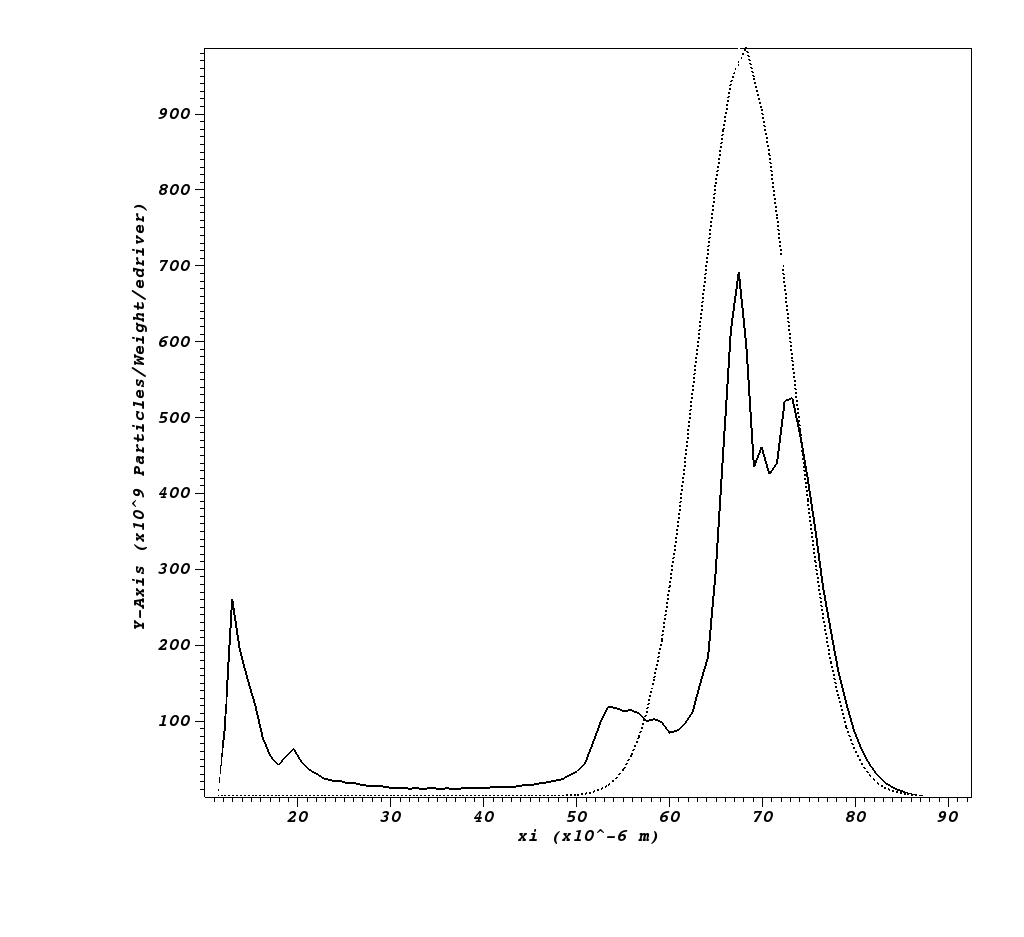
\includegraphics[width=0.66\textwidth]{25cm_lengthdist_start_end.png}\vspace{-20pt}\\
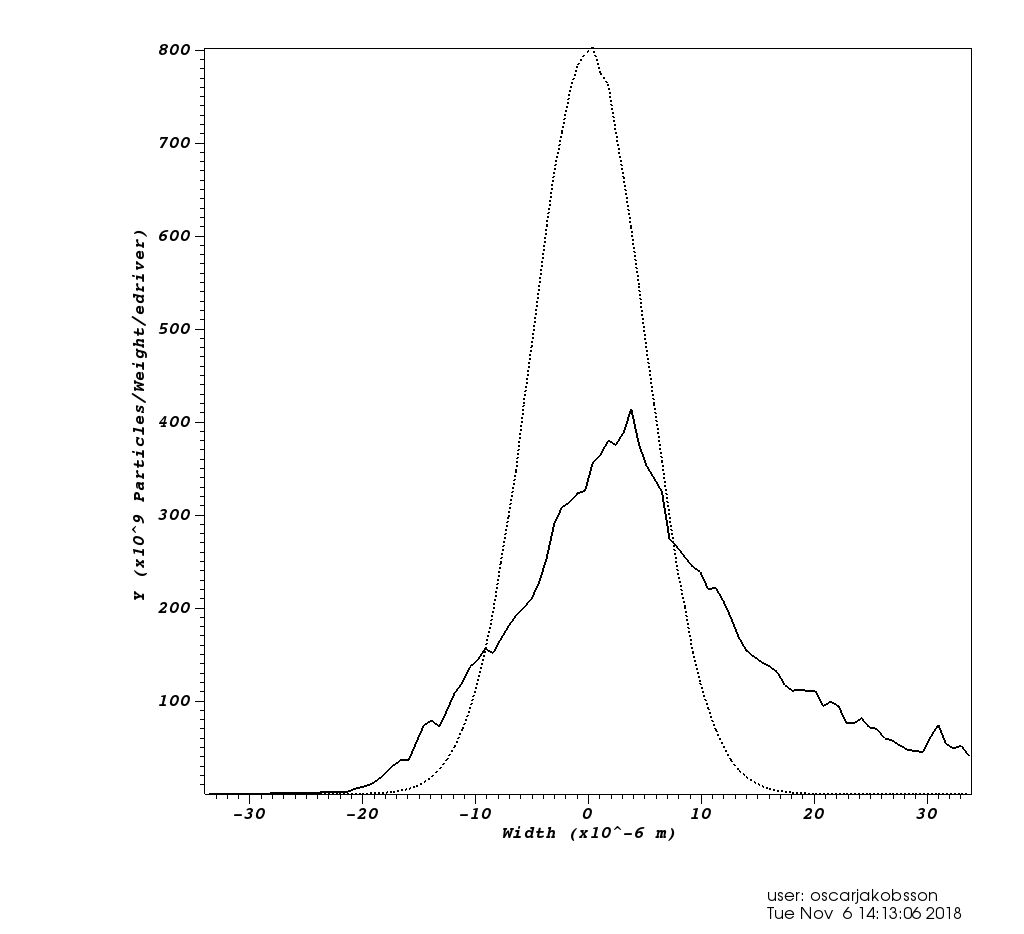
\includegraphics[width=0.66\textwidth]{25cm_widthdist_start_end.png}
\caption{{\textbf{(Left)}}{: Bunch length distribution for quasilinear case after propagating 0 cm (dotted) and 25 cm (solid)}. {\textbf{(Right)}}{: Bunch width distribution for quasilinear case after propagating 0 cm (dotted) and 25 cm (solid)}.}
\end{figure}

\clearpage


\noindent \textbf{Success!} Managed to set up an initial distribution with arbitrary energy distribution. 
\begin{figure}[!ht]
\centering
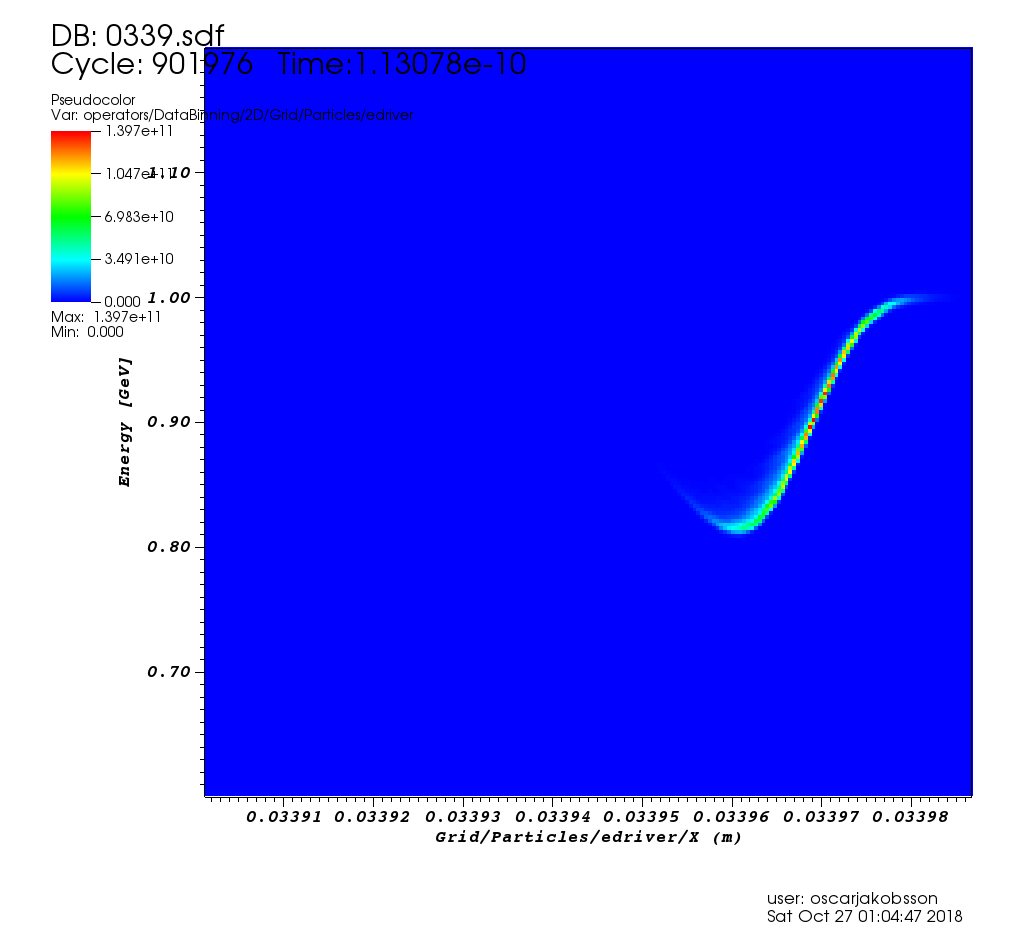
\includegraphics[width=0.49\textwidth]{visit0002.png}
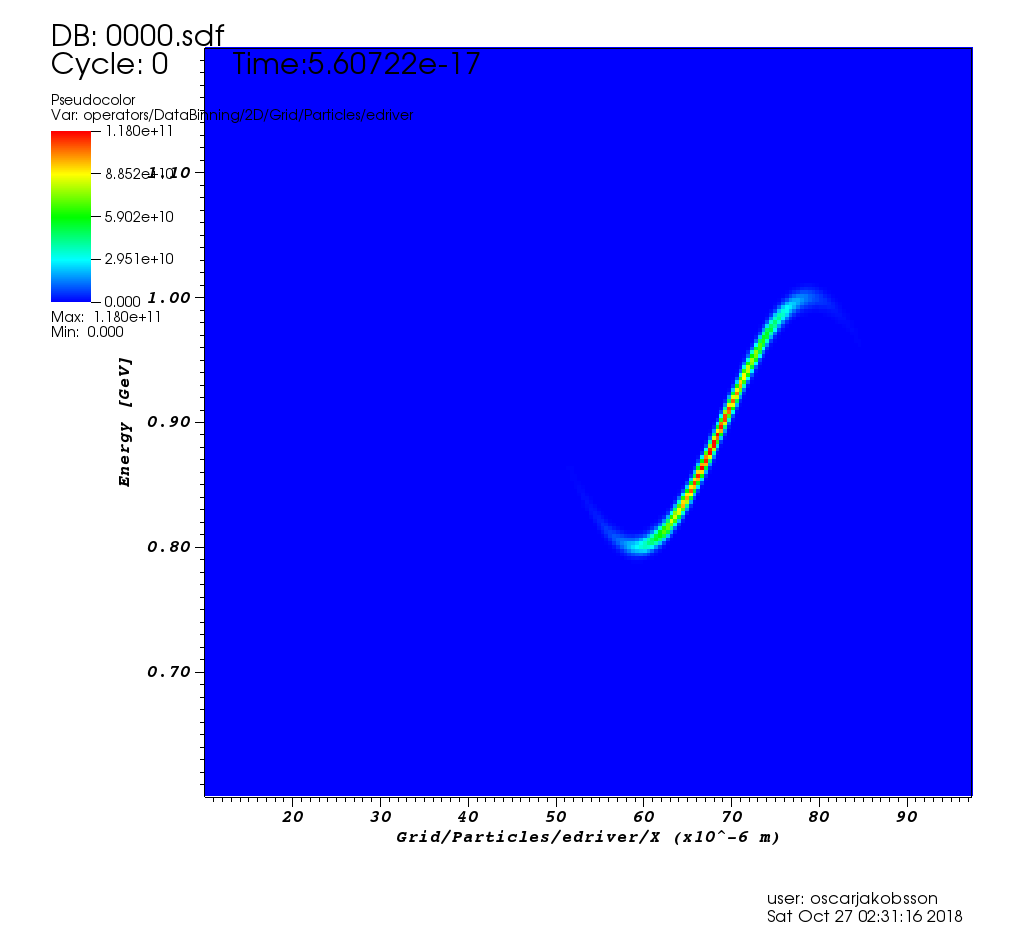
\includegraphics[width=0.49\textwidth]{visit0007.png}
\caption{\textcolor{Orange2}{\textbf{(Left)}}{: Energy distribution for bunch after propagating 3.4cm} \textcolor{blue}{\textbf{(Right)}}{: Energy distribution for bunch initialised at start of simulation.}}
\end{figure}
\begin{figure}[!ht]
\centering
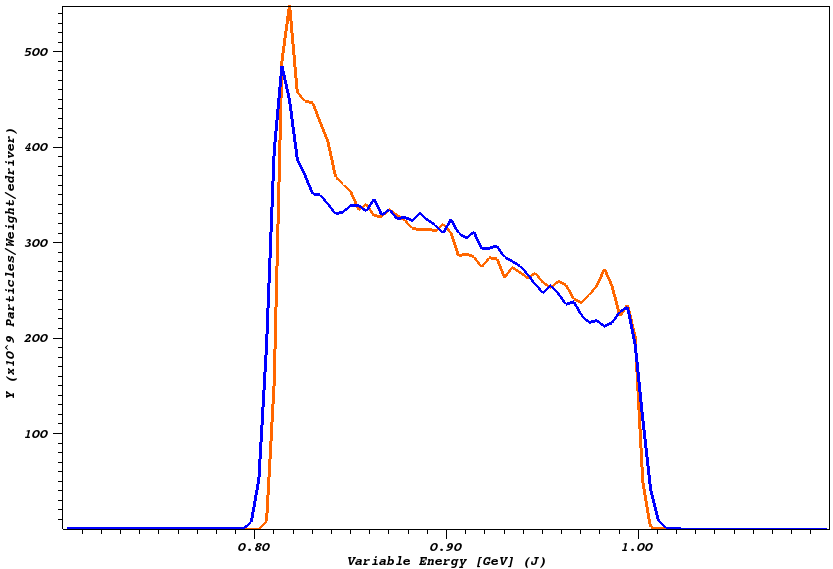
\includegraphics[width=0.8\textwidth]{visit0004.png}
\caption{\textcolor{Orange2}{\textbf{(1)}}{: Energy distribution for bunch after propagating 3.4cm} \textcolor{blue}{\textbf{(2)}}{: Energy distribution for bunch initialised at start of simulation.}}
\end{figure}

\clearpage
\section*{Laser tests}
Code to initalise a pre-saturated bunch 
\begin{lstlisting}
MODULE ic_module

  USE shared_data
  USE helper

  IMPLICIT NONE

  PRIVATE

  PUBLIC :: manual_load

CONTAINS

	SUBROUTINE manual_load
	  TYPE(particle), POINTER :: current
	  INTEGER, PARAMETER :: np_local = 1000
	  INTEGER :: ispecies, ip, i, nlines, IOstatus
	  REAL(num) :: temperature, stdev2, tail_width, tail_height, tail_drift
	  REAL(num) :: frac, tail_frac, min_p, max_p, dp_local, p2, tail_p2
	  REAL(num), DIMENSION(np_local) :: p_axis, distfn_axis
	  REAL(num) :: row, x, y, z, energy, weight
	  temperature = 1e15_num
	  tail_width = 0.05_num
	  tail_height = 9_num
	  tail_drift = 0.5_num
	  DO ispecies = 1, 1
	    stdev2 = kb * temperature * species_list(ispecies)%mass
	    frac = 1.0_num / (2.0_num * stdev2)
	    tail_frac = 1.0_num / (2.0_num * stdev2 * tail_width)
	    max_p = 7.0_num * SQRT(stdev2)
	    min_p = 0.5_num * max_p
	    dp_local = (max_p - min_p) / REAL(np_local-1, num)
	    DO ip = 1, np_local
			p_axis(ip) = min_p + (ip - 1) * dp_local
			p2 = p_axis(ip)
			tail_p2 = (p_axis(ip) - tail_drift * max_p)**2
			distfn_axis(ip) = EXP(-p2**2 * frac) * 0.5_num * (sign(1.0_num,4.8e-19_num-p2 )+1.0_num)


	    ENDDO
	    current=>species_list(ispecies)%attached_list%head

	    OPEN(UNIT = 17, FILE = "edriver_distributions.csv")

	    DO WHILE(ASSOCIATED(current))

			READ(17,*, end=10) row, x, y, z, energy, weight

			current%part_p(1) = energy/299792456
			current%part_pos(1) = x-0.279_num-62e-6_num  
			current%part_pos(2) = y
			current%weight = weight
   			current=>current%next


			!PRINT *, x
			!PRINT *, y
			!PRINT *, z
	    ENDDO
	    PRINT *, "Manual override - Loading custom particle distributions"
		5	format (f5.2,f5.2,f5.2,f5.2,f5.2,f5.2) 
		10	ClOSE(17)
	   ENDDO




	END SUBROUTINE manual_load


END MODULE ic_module
\end{lstlisting}
\begin{itemize}
\item Issue: restart not possible with laser. 
\item EPOCH allows for a user to manually override particle-parameter distributions defined in the input deck, in which all functions must be defined analytically. By overriding this so-called autoloader, which takes the analytical distributions in the input deck and distributes the macro particles accordingly, this manual approach allows for the initialisation of a bunch with non-analytical density and momentum distributions. 
\item Furthermore, even if the density distribution were to be easily described analytically, this method offers the advantage that it also overrides the maxwellian velocity distribution that epoch assigns to each bunch of particles in the input deck. This is fine for an initial bunch in thermal equilibrium, but as soon as plasma interaction occurs the velocity distribution of the electrons in the bunch is noticeably non-maxwellian
\item VisIt - export data from .sdf file, convert to -csv, read with ic module when compiling epoch.
\item (show below, it is possible to have a laser appear before the bunch at some time t, but the parameters of this laser could not be changed so testing several differnt laser intensities, distances etc. would take far too long if the bunch was forced to propagate 20cm each time before the laser was ramped up )
\end{itemize}
Use a time dependent laser bunch:
\begin{equation}
f(x,t)=\Theta\left(t-t_0\right)\exp\left\{\left(\frac{x-x_0}{w}\right)^2\right\}
\end{equation}
\begin{figure}[!ht]
\centering
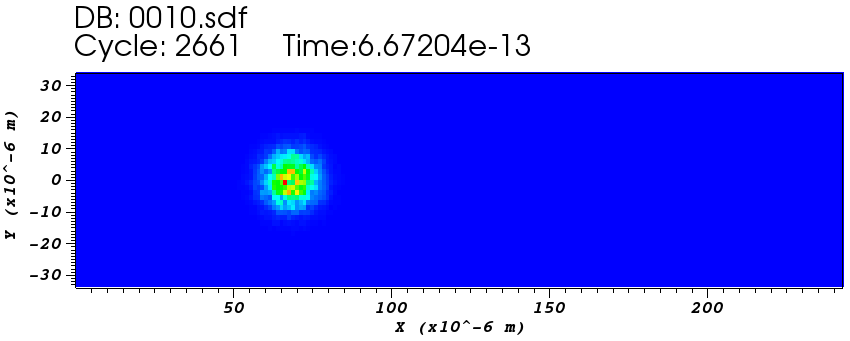
\includegraphics[width=0.7\textwidth]{buncht1copy.png}\\
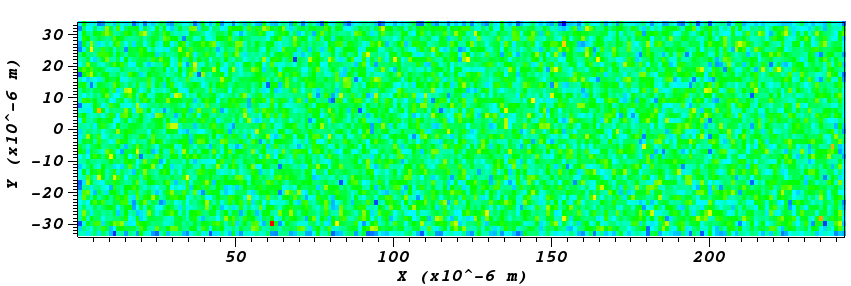
\includegraphics[width=0.7\textwidth]{lasert1copy.png}
\caption{Time: $t_1$. (Upper) edriver density, (Lower) electron plasma density}
\vspace{-10pt}
\end{figure}
\begin{figure}[!ht]
\centering
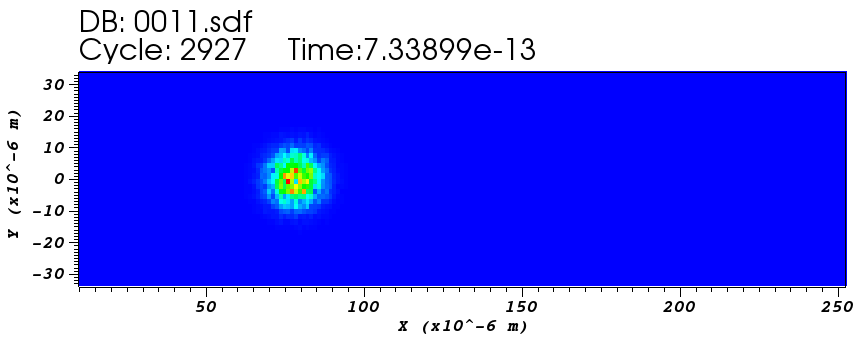
\includegraphics[width=0.7\textwidth]{buncht2copy.png}\\
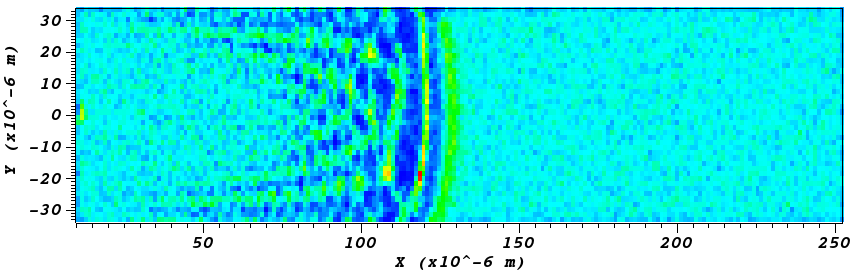
\includegraphics[width=0.7\textwidth]{lasert2copy.png}
\caption{SUCCESS! Time: $t_2$. (Upper) edriver density, (Lower) electron plasma density when laser has appeared at $\sim 120 \mu$m.  \textcolor{red}{Laser successfully initialised in front of bunch}}
\end{figure}
\clearpage
\subsection*{Plasma channel}
Still no success with the plasma channel. Dissipation continues despite the help of Bonatto. 
\begin{equation}
n_p(r)=\eta\frac{4r^2}{(k_pr_w)^4}
\end{equation} 
\begin{equation}
a(\xi,r)=a_0\exp(-\xi^2/\sigma^2_{\ell})\exp(-2r^2/r_w^2)
\end{equation}
\begin{figure}[!ht]
\centering
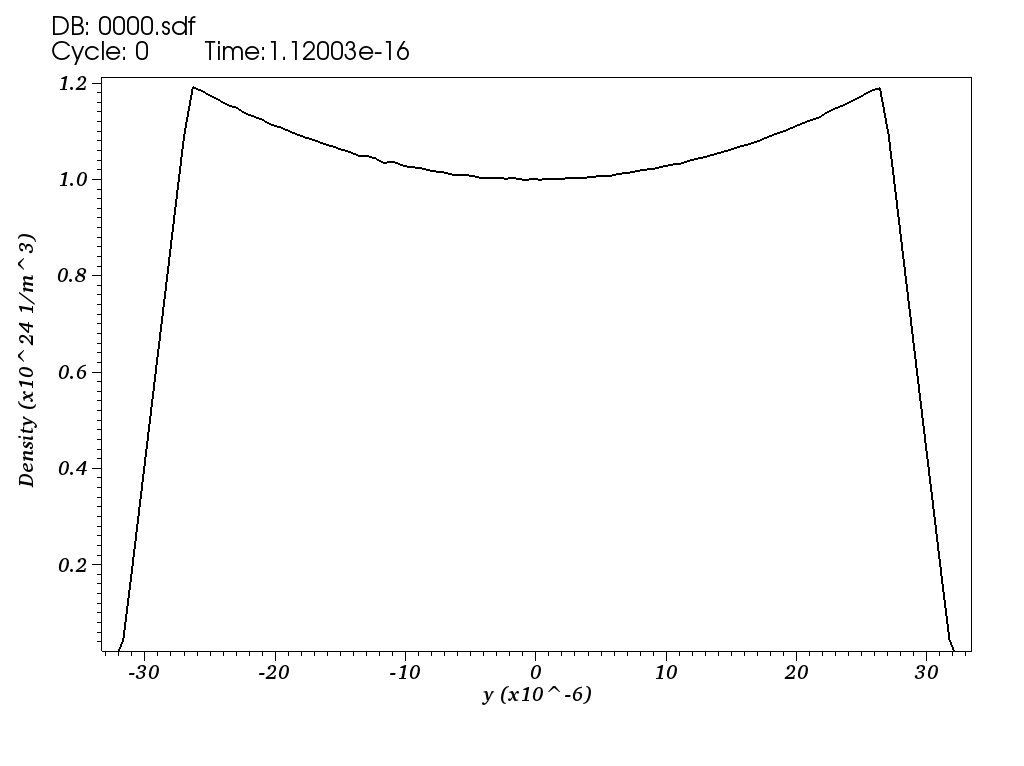
\includegraphics[width=0.5\textwidth]{visit0000.png}\\
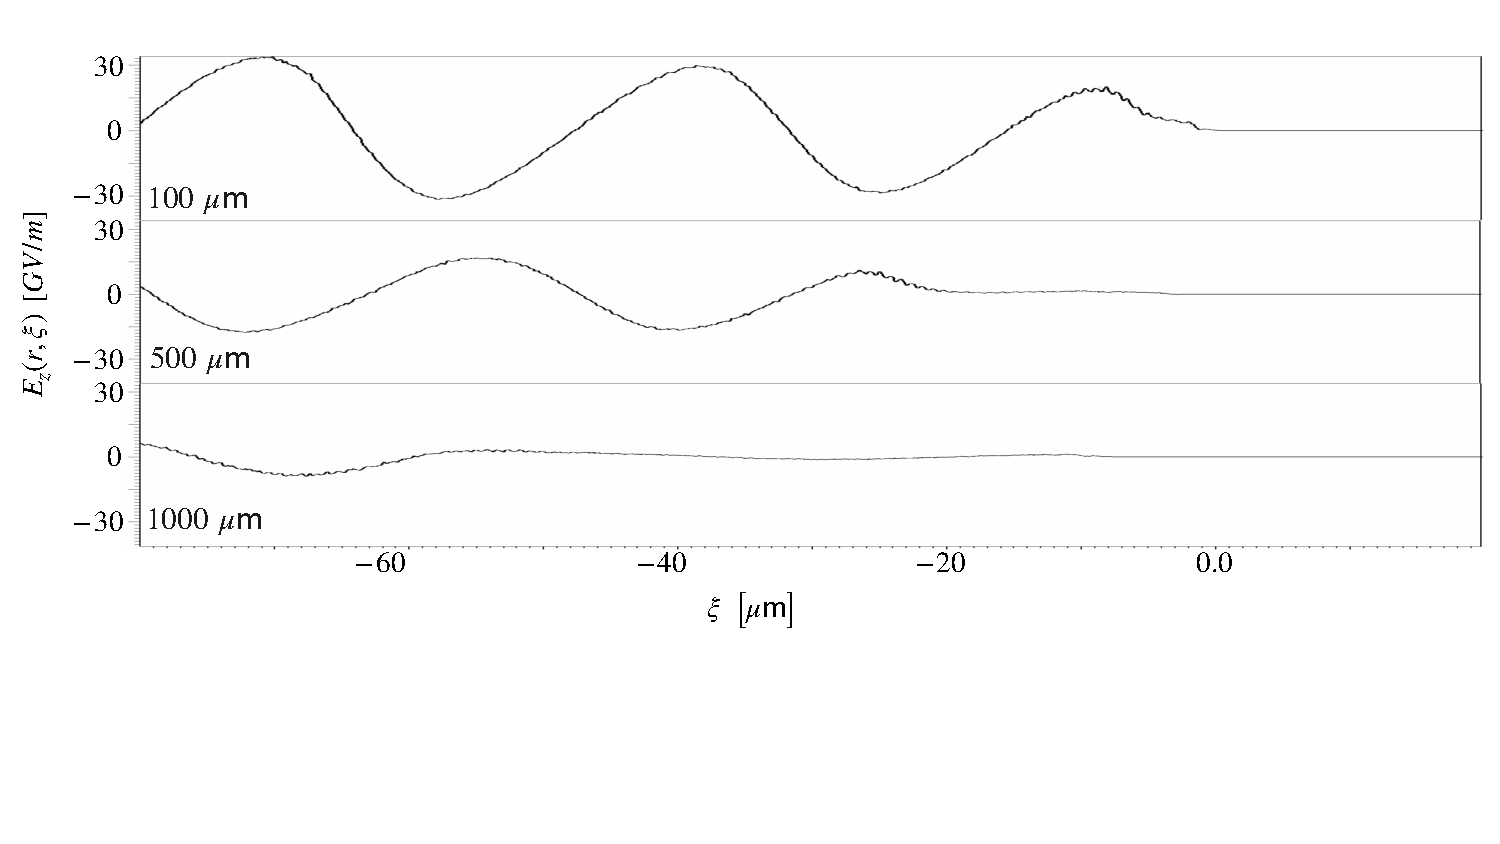
\includegraphics[width=0.8\textwidth]{laser}
\end{figure}





\clearpage
\subsection*{Notes.}
Meeting Guoxing:
\begin{itemize}
\item We will change $\sigma_{x,y}$, in simulation from $\sigma_{x,y}=0.3 \mu m ~\to~5-10 \mu m$ because the $0.3\mu m$ EuPRAXIA beam parameter gives to high beam density $n_b$, which means that we can't have $n_b\sim n_p$ because the plasma density would have to be too high. We should aim for $n_p\sim 10^{17}-10^{18}\sim n_b$ (standard L/PWFA) parameters. 
EuPRAXIA wants $\sigma_{x,y}$ small because small bunches gives more coherent radiation in undulators. One could expand the beam by letting it propagate freely (expand due to space charge) a distance before reaching the beam dump. 
\item $\text{Run simulations with uniform plasma density for }\left\{\begin{aligned}
&n_p\sim 0.1 n_b \quad &&\text{Non-linear}\\
&n_p\sim  n_b\quad &&\text{Quasi-linear}\\
&n_p\sim 10 n_b\quad &&\text{Linear}
\end{aligned}\right.$ \\
\item Use $\Delta E/E=0.01$ and bunch charge $30~$pC ($5~$fs).\\
\item Estimate necessary simulation propagation length by saturation length using wave-breaking electric field gradient 
$$L_{\text{sat}}\approx \frac{T_0}{eE_{wb}}=\frac{T_0}{e}\frac{e}{m_e c\omega_p}=\frac{T_0}{m_e c}\sqrt{\frac{m_e e\epsilon_0}{e^2n_b}} $$ 
\item Project outline:
\begin{itemize}
\item Uniform plasma with varying $n_b\sim n_p$
\item Vary plasma density profile
\item Test laser to dump head of beam
\item Run simulations for real FlashForward parameters and not the idealized EuPRAXIA parameters.
\end{itemize}
\item  100pC $$n_b=\frac{N_p}{(2\pi)^{3/2} \sigma_y^2\sigma_x}=\frac{6.25\times 10^{8}}{(2\pi)^{3/2} (5\times 10^{-6})^3}\approx 3.2\times 10^{23}~ \text{m}^{-3} $$
$$\Rightarrow ~~eE_{\text{wb}}=\left\{\begin{aligned}
&17 ~\text{GeV/m }&& n_p=0.1 n_b \\
&54 ~\text{GeV/m} && n_p=n_b\\
&172 ~\text{GeV/m} &&n_p=10 n_b
\end{aligned}\right.\quad\Rightarrow ~~L_{sat}(1 ~\text{GeV})=\left\{\begin{aligned}
&5.8 ~\text{cm}&& n_p=0.1 n_b \\
&1.9 ~\text{cm} && n_p=n_b\\
&0.6 ~\text{cm} &&n_p=10 n_b
\end{aligned}\right.$$
$$1 ~\text{GeV beam} ~~\Rightarrow ~~ L_{sat}\sim 2 ~\text{cm}=2*10^4 \mu \text{m} $$
\item  30pC $$n_b=\frac{N_p}{(2\pi)^{3/2} \sigma_y^2\sigma_x}=\frac{1.87\times 10^{8}}{(2\pi)^{3/2} (5\times 10^{-6})^3}\approx 9.5\times 10^{22}~ \text{m}^{-3} $$
$$\Rightarrow ~~eE_{\text{wb}}=\left\{\begin{aligned}
&9.4 ~\text{GeV/m }&& n_p=0.1 n_b \\
&30 ~\text{GeV/m} && n_p=n_b\\
&94 ~\text{GeV/m} &&n_p=10 n_b
\end{aligned}\right.\quad\Rightarrow ~~L_{sat}(1 ~\text{GeV})=\left\{\begin{aligned}
&10.7 ~\text{cm}&& n_p=0.1 n_b \\
&3.4 ~\text{cm} && n_p=n_b\\
&1.1 ~\text{cm} &&n_p=10 n_b
\end{aligned}\right.$$
$$1 ~\text{GeV beam} ~~\Rightarrow ~~ L_{sat}\sim 3.4 ~\text{cm}=3.4*10^4 \mu \text{m} $$

\end{itemize}




\subsection{Input deck}
Once EPOCH has been downloaded and compiled the so-called input deck is essentially EPOCH's user interface. This is a file in which users specify the details of a simulations and it is this file that gets read by EPOCH and passed onto the core PIC algorithm. The input deck consists of blocks which define parameters for different features of the simulation. \\
\textbf{Explain control block first}, and what the restart does.
\begin{verbatim}
begin:control
  dlb_threshold = 0.5
  restart_snapshot=restartXXXX.sdf
  t_end = end_time
  nx = nint(length / cell_length)
  ny = nint((half_width * 2) / cell_width)
  npart = part_per_cell * nx * ny
  stdout_frequency = 50
  use_random_seed = T
end:control
\end{verbatim}
This specifies the grid that the simulations is to run on. We then populate this grid with plasma particles.
\textbf{Species block}, with explanation about analytical density distributions for plasma, and specify ppc.\\
The control and species blocks together define the resolution of the simulation. When setting up the resolution of the grid one has to make sure that the grid is sufficiently fine such that the smallest features of our physical system are resolved. This is to ensure that the simulation accurately models the physical system it is meant to represent, to the extent that missing small scale phenomena might alter the large scale outcome of the simulation. A finer grid however requires more macroparticles to fully populate the grid, which inevitably extents the computational time. In addition the time step $\Delta t$ aneeds to be suitably decreased as well. This is because of the so-called Courant-Friedrichs-Lewy (CFL) condition.  Any simulation introduces uncertainties in the final outcome due to the finite resolution. We need to make sure that the uncertainties introduces during each iteration do not build up and grow unbounded. \\
\\
\textbf{edriver} with analytical distribution, and laser, followed by boundaries
\begin{center}
\begin{verbatim}
begin:boundaries
  bc_x_min = simple_laser
  bc_x_max = simple_outflow
  bc_y_min = simple_outflow
  bc_y_max = simple_outflow
end:boundaries
\end{verbatim}
\end{center}
\textbf{output block} and the sdf file visualisation with VisIT








\clearpage
 \vfill
 \bibliographystyle{unsrt}
 \bibliography{PWFA.bib}


 \end{document}
 